\documentclass[twoside, 12pt, letterpaper]{report}\usepackage[]{graphicx}\usepackage[]{color}
% maxwidth is the original width if it is less than linewidth
% otherwise use linewidth (to make sure the graphics do not exceed the margin)
\makeatletter
\def\maxwidth{ %
  \ifdim\Gin@nat@width>\linewidth
    \linewidth
  \else
    \Gin@nat@width
  \fi
}
\makeatother

\definecolor{fgcolor}{rgb}{0.345, 0.345, 0.345}
\newcommand{\hlnum}[1]{\textcolor[rgb]{0.686,0.059,0.569}{#1}}%
\newcommand{\hlstr}[1]{\textcolor[rgb]{0.192,0.494,0.8}{#1}}%
\newcommand{\hlcom}[1]{\textcolor[rgb]{0.678,0.584,0.686}{\textit{#1}}}%
\newcommand{\hlopt}[1]{\textcolor[rgb]{0,0,0}{#1}}%
\newcommand{\hlstd}[1]{\textcolor[rgb]{0.345,0.345,0.345}{#1}}%
\newcommand{\hlkwa}[1]{\textcolor[rgb]{0.161,0.373,0.58}{\textbf{#1}}}%
\newcommand{\hlkwb}[1]{\textcolor[rgb]{0.69,0.353,0.396}{#1}}%
\newcommand{\hlkwc}[1]{\textcolor[rgb]{0.333,0.667,0.333}{#1}}%
\newcommand{\hlkwd}[1]{\textcolor[rgb]{0.737,0.353,0.396}{\textbf{#1}}}%
\let\hlipl\hlkwb

\usepackage{framed}
\makeatletter
\newenvironment{kframe}{%
 \def\at@end@of@kframe{}%
 \ifinner\ifhmode%
  \def\at@end@of@kframe{\end{minipage}}%
  \begin{minipage}{\columnwidth}%
 \fi\fi%
 \def\FrameCommand##1{\hskip\@totalleftmargin \hskip-\fboxsep
 \colorbox{shadecolor}{##1}\hskip-\fboxsep
     % There is no \\@totalrightmargin, so:
     \hskip-\linewidth \hskip-\@totalleftmargin \hskip\columnwidth}%
 \MakeFramed {\advance\hsize-\width
   \@totalleftmargin\z@ \linewidth\hsize
   \@setminipage}}%
 {\par\unskip\endMakeFramed%
 \at@end@of@kframe}
\makeatother

\definecolor{shadecolor}{rgb}{.97, .97, .97}
\definecolor{messagecolor}{rgb}{0, 0, 0}
\definecolor{warningcolor}{rgb}{1, 0, 1}
\definecolor{errorcolor}{rgb}{1, 0, 0}
\newenvironment{knitrout}{}{} % an empty environment to be redefined in TeX

\usepackage{alltt}

%%%Packages
\usepackage[margin=1in]{geometry}
\usepackage{multicol}
\setlength{\columnsep}{1cm}
\usepackage{newpxtext,newpxmath}
\usepackage{hyperref}
\usepackage{lipsum}
\usepackage{tocloft}
\usepackage{xcolor}
%\usepackage{comment}
\usepackage{framed}
\renewcommand{\cftpartleader}{\cftdotfill{\cftdotsep}} % for parts
\renewcommand{\cftchapleader}{\cftdotfill{\cftdotsep}} % for chapters
\renewcommand{\cftsecleader}{\cftdotfill{\cftdotsep}}


%%%%Title Info
%\author{}
%\title{The Mechanician\{s\} World \newline Compendium for Role-Player's}
%\date{}
\IfFileExists{upquote.sty}{\usepackage{upquote}}{}
\begin{document}

%%%%Custom Commands
\newcommand{\npart}[1]{\part*{#1} \addcontentsline{toc}{part}{#1}}
\newcommand{\nchapter}[1]{\begin{framed} \chapter*{#1} \addcontentsline{toc}{chapter}{#1} \end{framed}}
\newcommand{\nsection}[1]{\section*{#1} \addcontentsline{toc}{section}{#1}}
\newcommand{\nsubsection}[1]{\subsection*{#1} \addcontentsline{toc}{subsection}{#1}}
\newcommand{\nsubsubsection}[1]{\subsubsection*{#1} \addcontentsline{toc}{subsubsection}{#1}}
\newcommand{\nparagraph}[1]{\paragraph*{#1} \addcontentsline{toc}{paragraph}{#1}}
\newcommand{\nsubparagraph}[1]{\subparagraph*{#1} \addcontentsline{toc}{subparagraph}{#1}}

\newcommand{\nmw}{\textit{Mechanician\{s\} World }}
\newcommand{\mw}{\nmw}
\newcommand{\ooi}{on/in }


\newcommand{\cat}{Rubifol'} %1
\newcommand{\tarsier}{Tarsifol'} %2
\newcommand{\hopper}{Hopper's} %3
\newcommand{\mantis}{Manti's} %4
\newcommand{\mech}{Machinefol'} %5 have several types of machineFol' that more or less constitute their own races.
\newcommand{\rat}{Ratfol'} %no rat Fol' anymore, rats went extinct in a war between the rats and the mice. Not all rats were bad, but a select few were. Rats had enslaved the mice, though the mice greatly outnumbered the rats. The Mice revolted by using a biochemical weapon that decimated the entire species, or so it goes. Whether they still survive is up to speculation. The rats are villainized for it in historical text and the publics eye.
\newcommand{\mouse}{Mousefol'} %6
\newcommand{\mole}{Molefol'} %7
\newcommand{\owl}{Owlfol' } %will take the place of dragons. both wild and as pets/mounts.
\newcommand{\hnbat}{Hognose }  %8
\newcommand{\vmbat}{Leafnose } %9
\newcommand{\ftbat}{Beastnose } %10
\newcommand{\rabbit}{Rabbitfol' } %11
\newcommand{\hedgehog}{Heygfol' } %12
\newcommand{\squirrel}{Pumifol' } %13
\newcommand{\marmoset}{Cebufol' } %14
\newcommand{\possum}{Pedufol'} %15
\newcommand{\glider}{Lumbalkfol'} %16

%newcommand{\spoiler}[1]{}
\newcommand{\spoiler}[1]{\textcolor{purple}{#1 }}
\newcommand{\fourthwall}[1]{#1 }


%%%%

\begin{center}
\begin{framed}
\Huge{The}

\Huge{\nmw}

\Huge{Compendium for Role-Player's}

\end{framed}
\end{center}
\newpage

\chapter*{Credits}

\newpage

\tableofcontents

\newpage
\nchapter{Preface}
This setting has been in development in one way or another for at least six years. The name 'Mechanician' has been attached to it for at least three of those years. I am not nearly dedicated enough and I have heard on numerous occasions---from none other than myself---that I simply do not have the time to develop my skill in fiction writing to the point where I could craft a fully functioning story that I am proud of (whether or not that would ever be possible is up for debate [one with a skilled therapist would probably be most beneficial]; maybe in the distant future I will less match the profile of an ADHD poster-child... or poster-man, I suppose). On the other hand, I have already thought my way through a large majority of a sliver of the \mw setting and I figure it would be a shame to not build further upon it while also trying to utilize it in some fashion: I have attempted such a feat numerous times, here is the latest.

I have drawn inspiration from all over the fucking place. Some ideas are more original than others, all have been done before, which is unavoidable. Hopefully the mish-mash I am brewing is a somewhat interesting and proprietary blend. If I were to take my best shot at a single sentence description, without taking any time to sound original or profound, it would be "The Borrowers establish societies of their own in the ruins of humanity, featuring surprisingly sentient AI and not entirely but sort-of pretty-much magic and sewage system highways leading to sprawling underground cities and domesticated arthropods that would seem pretty big to someone standing at only two inches tall and mechanical cats and talking rats and other stuff." Sounds good to me. If anyone ever sees this, hope you enjoy.

\vspace{1cm}
Cheers,

Nathan

\begin{multicols*}{2}
\end{multicols*}
\newpage

\nchapter{Introduction}
\begin{multicols*}{2}
This book is intended as a complete reference and guide for DM's and players looking to explore the home-brewed \nmw setting. This game has been built via inspiration from various prior game systems including the Dungeons \& Dragons 5e rule-system as found in the System Reference Document 5.1 (SRD). Only content which satisfies the requirements of the Open Game License Version 1.0a under which the SRD was published have been incorporated.

This is not only a guide to the \nmw setting, featuring various world-building details, but covers all aspects of gameplay including character building and the rules of the game. \textbf{No other source materials are required to play the contained game, though physical or virtual variants of a pen and pad of paper, set of typical RPG dice, and so on are required.} 

Those familiar with DnD 5e may notice that some mechanics have been retained without modification, while others have been tweaked (if only by name to better fit the \nmw). In some cases mechanics have been signficantly overhauled or left out entirely.

The rule-system was drafted with a few goals in mind:
\begin{itemize}
\item Keeping things simple, silly.
\item Toning down magic a bit.
\begin{itemize}
\item Removing spells which don't fit the theme or don't make sense given the worlds 'physics'.
\item Removing spells which would make one 'god-like'.
\item Adjusting spell stat's.
\end{itemize}
\item Making sure it fits the lore. This applies to many topics.
\item Making battle feel a bit more gritty and dangerous while also encouraging creativity and action. I ti sokay to hide every once in a while, as well as go out on a limb.
\item Making sure 'races' feel like more than just humans of greatly varying height and stature. Species should feel unique and offer fun abilities that set them apart in a way which makes sense given their background, physiology, and so on.
\item Retooling classes to only those which make sense. 
\item Reducing the emphasis on classes in order to open up possibilities for players in battle. Choices such as race, backstory, and anything which adds to a characters depth is encouraged, whereas anything which pigeonholes a player and reduces their opportunity to act as their hearts and imaginations desire are given a second thought. Everyone should feel like special little heroes (pinches ones cheek) because they have their own interesting experiences and strategies to bring to the table. As such, less worry has been wasted on crafting perfect balance between races and classes in order to counteract min-maxer's (players that like to minimize character faults and maximize performace to create the most powerful character possible.). The game is meant to be enjoyed and to allow shared creativity, not facilitate a grind to the top. It is the DM's job to find ways to uniquely challenge any players which may be a bit OP'd. Despite that, some effort has been made to make sure any character building choices won't lead to massively disproportiantely over-powered characters relative to others.
\item Encouraging cooperation, assists, and teamwork in battle. 
\item This system is more focused on the story and the roles players are enagegd in. A fun and memorable experience is most important. We try to avoid mechanics which rely solely on immediate gratification such as grinding for experience and hording loot. Gear is fun, but it should aid in the journey, not be the focus. Further, sneaking around or hiding in the shadows as enemies pass by is a legitimate strategy which adventurers would arguably improve upon with practice. Following this train of thought, we have removed the concept of experience entirely. Players need not worry about how close they are to the next level and certainly shouldn't decide whether or not to ambush an unsuspecting enemy simply because they need the 250xp that they would gain.
\item Make characters feel useful from the start. It shouldn't take until at least level 5 or more before it becomes fun to play your character. Of course character progressions are important, though progress and victories can be rewarded and signified in other ways aside from experience dumps and the long slog to level 20. 
\item Keeping the game running at a pace that limits player boredom, partly by removing unnecessary mechanics which don't seem to add much depth or fun as is (looking at you Pathfinder).
\end{itemize}
\nsection{Using This Book}
This compendium has been designed as a one-stop manual for both DM's and players. The Lore and events discussed in this manual are far from exhaustive and in fact only cover a very minor portion of happenings on the \mw. This information will be expanded upon with time, though at no point will we cover more than a sliver of the happenings \ooi the \mw. Why is this you might ask?: because I am too indecisive to decide when enough is enough. The information provided covers some of the most significant events and happenings (that I have contrived so far), often those which apply to the \mw as a whole and which help establish the look and feel (and smell and taste for that matter) of the \mw. All sections of this book are relevant to DM's, whereas all sections apart from \textit{one}, the \textbf{'What to Expect While \ooi the \mw'} section, are relevant to players. This DM-only section includes detailed world-building that more than likely contains details best experienced in-game, i.e., spoilers. I have placed this spoiler heavy section at the very back of the book and included some very threatening red font to ward away voyeurs and other flavors of party-pooper. The lore and trivia I have deemed important to players prior to their first formal experience in the \mw is contained in a short primer at the very start of the book. It contains only the information crucial to understanding the \mw, the sort of information all denizens would be privy to and which is likely important in character creation and role-playing and overall helps avoid confusion. I have tried my best to keep this primer as short as possible. Some other world-building information is divulged to players selectively through the character-building process.  


The rest of the book is dedicated to covering the mechanics of the game itself, starting with character building and moving along through the nitty-gritty rules important to adventuring and combat. We then include materials players and DM's might need to refer to repeatedly, including common inhabitants one might run into \ooi the \mw, magic spells some might wield, conditions one might bestow or receive (for better or worse) as well as a Glossary of common used terms, some helpful maps of the \mw: \ooi, and quick synopses for various mechanics that might make things run a bit more smoothly mid-game. Again, the very back is off limits unless you are an aspiring or proven DM, or unless your DM says otherwise.

\nsection{How to Play}
Players and DMs ought to initially read through front to back (or nearly to the back for players). These sorts of games always require a bit of pre-game homework. I have tried to keep that work as quick and painless as possible. 

The play of the game unfolds according to this basic pattern. 1. The DM describes the environment. The DM tells the players where their adventurers are and what's around them, presenting the basic scope of options that present themselves (how many doors lead out of a room , what's on a table, who's in the tavern, and so on).

The players describe what they want to do. Sometimes one player speaks for the whole party, saying, "We'll take the east door," for example. Other times, different adventurers do different things: one adventurer might search a treasure chest w hile a second exam ines an esoteric symbol engraved on a wall and a third keeps watch for monsters. The players don't need to take turns, but the DM listens to every player and decides how to resolve those actions. Sometimes, resolving a task is easy. If an adventurer wants to walk across a room and open a door, the DM might just say that the door opens and describe what lies beyond. But the door might be locked, the floor might hide a deadly trap, or som e other circum stance might make it challenging for an adventurer to complete a task. In those cases, the DM decides what happens, often relying on the roll of a die to determine the results of an action. 3. The DM narrates the results of the adventurers' actions. D escribing the results often leads to another decision point, which brings the flow of the game right
 back to step 1.

This pattern holds whether the adventurers are cautiously exploring a ruin, talking to a devious prince, or locked in mortal combat against a mighty dragon. In certain situations, particularly combat, the action is more structured and the players (and DM) do take turns choosing and resolving actions. But m ost of the time, play is fluid and flexible, adapting to the circumstances of the adventure. Often the action of an adventure takes place in the imagination of the players and DM, relying on the DM 's verbal descriptions to set the scene. S om e DMs like to use music, art, or recorded sound effects to help set the mood, and many players and DMs alike adopt different voices for the various adventurers, monsters, and other characters they play in the game. Som etim es, a DM might lay out a map and use tokens or miniature figures to represent each creature involved in a scene to help the players keep track of where everyone is.

Example of DnD roleplaying.
\end{multicols*}

\part*{Welcome}
\nchapter{Primer: The Game}
\begin{multicols*}{2}
\nsection{Dice}
The only dice used is the d10. The Abilities determine how many dice you can roll and the Skills determine the range of values you need to roll. The more skilled you are, the lower dice value is necessary.
\nsection{Character Creation}
\nsection{Profession}
\nsection{Abilities}
\nsection{Skills}
\nsection{Focus Points}
\nsection{Skill Rolls}
\nsection{Success, Failure, and Fumble}
\end{multicols*}
\nchapter{Primer: Critical Features of the \mw}
\begin{multicols*}{2}
Unlike many RPG settings where human homologues with pointy ears and atypical skin tones inhabit an otherwise Tolkein-esque setting, the \mw diverges in ways that only make sense to point-out prior to your first game-session. This chapter is meant to help players get into the mindspace of the \mw as quickly and painlessly as possible so that all parties involved can hit the ground running. 
\nsection{Familiar World}
In the not-too-distant future a mysterious catastrophic event of unknown origin has effectively extinguished much of the animal life on Earth. Those affected, collectively referred to by the various contemporary sentient denizens of Earth as the 'Static', remain frozen in place in their final unaware acts. The Static are hardened to the touch and appear to be highly resistant to the wear and tear of time and the elements. While they have remained mostly unscathed over several thousand years, the planet has continued to change around them, often incorporating them into the landscape to where in some cases it can be difficult to distinguish between mossy mound and what was once a fleshy, furry, feathery, or scaley protuberance.
\nsection{On the Static}
While much is unknown regarding the nature and origin of the Static, a few facts seem to hold true: 1) Only Animalia appear to have been affected, 2) if a member of a species was affected all members of that species were affected, and 3) a novel hypothesis known as "blanks window" explains the likelihood of an organism having been affected based on the organisms mass: following a linear probability distribution species at the center of the distribution have a 50\% likelihood of being affected; as an organisms mass falls below the center of the distribution the likelihood of having been affected drops significantly until the mass reaches a lower limit of blanks window wherin the likelihood of being affected is effectively 0\% and as an organisms mass grows above the center of the distribution the likelihood of having been affected rises significantly until the windows upper-limit is reached at which point the likelihood of being affected is effectively 100\%.

\nsection{Novel Point-of-View}
Contemporary sentient beings, in many ways similar to humankind, have filled the void humans left behind (these beings will be collectively referred to henceforth as 'denizens'). In fact the denizens of the \mw have gone a step further, filling many of the crags, cracks, and crannies humans often overlooked simply because they couldn't fit. Societies flourish and fail on an entirely new scale, with the average standing height of denizens ranging between 3 to 10 cm's.

For a variety of reasons we will discuss later, most civilizations have taken refuge underground, filling in natural cave systems, hollowing out the Earth in order to expand, and utilizing what remains of the infrastructure left behind by mankind.

\nsection{Robust and Varied Denizens}
A number of distinct sentient denizens (races) have forged new homes and societies \ooi the \mw. In some cases denizens of different races have intermingled, created diverse new civilizations: this doesn't mean they always get along. Others choose to remain isolated, each with their own reasons. Others yet have simply never crossed paths with one of the many rapidly expanding civilizations. Despite the variety in races and cultures which has arisen since the Static, the similarities these new denizens share with humankind are uncanny, though these denizens have very little understanding as to just how similar they really are, much less why that might be.

\nsection{Opinions Abound}
History is fuzzy: opinions are varied and abundant on just what the Static are and whether they are best described as a what or a who, or, for that matter, whether they should be worshipped, studied, harvested, left alone, or even avoided like a plague. Unfortunately, the keenest minds have made little progress is uncovering the secrets of the past. It is clear that past societies had inhabited much of the Earth, and that the gargantuan bipedal Static (humans) seem to be closely linked, though little more is understood and even that much is enough to start a heated debate or, in some cases, get yourself killed. While most everyone may subscribe to one hypothesis or another, those that espouse their particular flavor of events range from casual gossips to religious zealots: indeed many religions and cults have formed around the mysteries of the past, each attempting to explain not only the nature and origin of the Static but all aspects of existence on the \mw. Where the truth lies amongst the heaps of opinions struggling to reach the top may never be known, though it may go without saying that some opinions are closer to the truth than others. These are pioneering times on the \mw and with that brings mysteries and often poor reasoning skills. Often sound reasoning and evidence holds less wieght than it ought to, as is true of the inverse, poor reasoning and evidence is given greater credence than it ought to. 
\nsection{Technology}

\nsection{Magic}
\end{multicols*}



\nchapter{Building a Character for the \nmw}
\begin{multicols*}{2}
\nsection{Varieties of Fol' \ooi the \mw}
The planet Earth is massive. \fourthwall{It felt so to most humans and it certainly would seem so to the small statured Fol' of the \mw. Not all animals were affected by the Static, and among those that weren't, a puzzling number have developed impressive cognitive capacities. The Fol' which make up the largest group on Earth are the \mech's, though their organic counterparts have been repidly catching up. All playable Fol' in the \mw are at least capable of upright bipedal movement, freeing their quite capable arms for action. To be honest, bipedal isn't entirely accurate, since some Fol' may be pacing around the \mw with more than two legs, but you get the idea. The Fol' of the \mw have classified themselves into five taxonomies, though these folk classifications appear to be driven solely upon physical similarities, tradition, and myth as opposed to phylogenetic relation. Origin stories abound for all Fol', some more flattering than others and some more accurate than others. The commonly held classifications of Fol' include: 1) Mechanical, 2) Insectoid, 3) Bat, and 4) Critters. We are currently aware of the following Fol', or sentient beings, found \ooi the \mw:}
\nsubsubsection{Mechanical}
\nparagraph{\mech}
Mechanical beings resembling humanoids in may ways. Highly adaptable and found in many roles.
Presence: \mech make up the largest proportion of Fol'. Estimated 35 to 45 percent of regional population. 
\nsubsubsection{Insectoids}
\nparagraph{\hopper}
Humanoids decinded from grasshoppers.
\nparagraph{\mantis}
Humanoids decinded from Mantises.
\nsubsubsection{Bats}
\nparagraph{\hnbat}
Humanoids decinded from small insectovore bats.
\nparagraph{\vmbat}
Humanoids decinded from vampire bats. Lives on blood.
\nparagraph{\ftbat}
Humanoids decinded from fruit bats.
\nsubsubsection{Critters}
\nparagraph{\tarsier}
Humanoids decinded from Tarsiers.
\nparagraph{\marmoset}
Humanoids decinded from Marmosets.
\nparagraph{\mouse}
Humanoids decinded from Mice.
\nparagraph{\mole}
Humanoids decinded from Moles.
\nparagraph{\squirrel}
Humanoids decinded from pygmy-squirrels.
\nparagraph{\rabbit}
Humanoids decinded from dwarf rabbits.
\nparagraph{\cat}
Humanoids decinded from felines.
\nparagraph{\hedgehog}
Humanoids decinded from Hedgehogs.
\nparagraph{\possum}
Humanoids decinded from Tasmanian Pygmy Possum.
\nparagraph{\glider}
Humanoids decinded from Sugar Gliders.
\end{multicols*}
\begin{center}
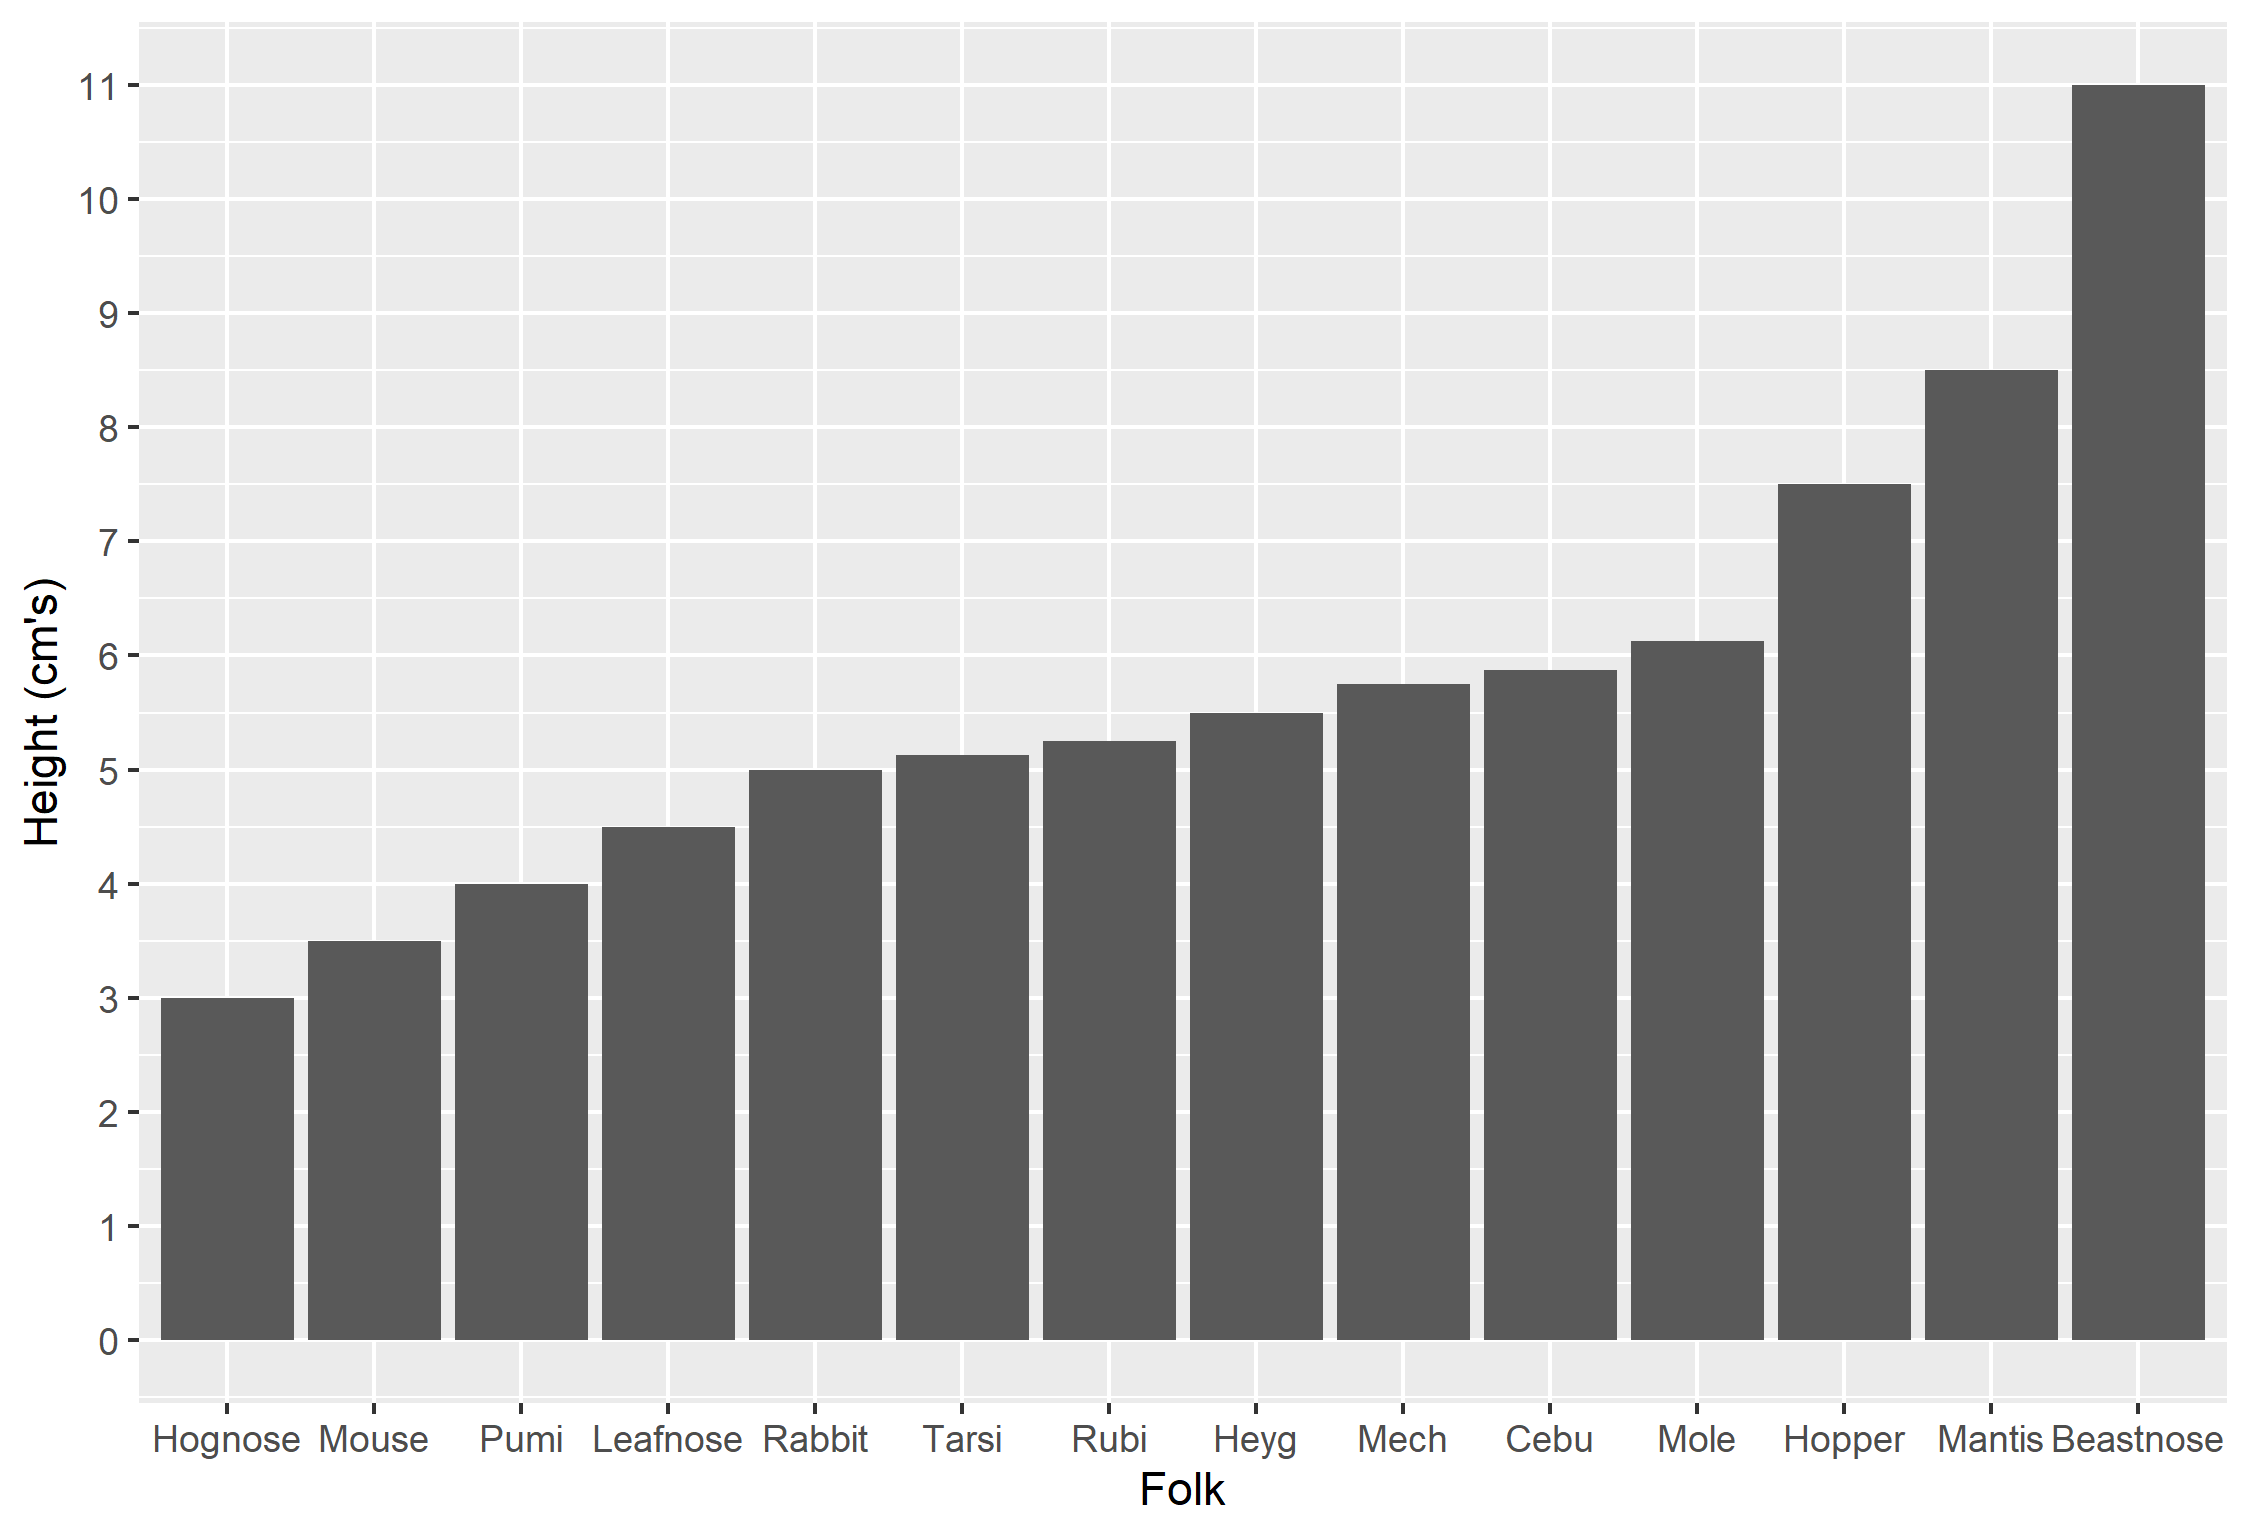
\includegraphics{PC_heights_chart.png}
\end{center}
\begin{multicols*}{2}
\nsubsection{\mech}
The most human-like of all Fol' and also among the most-diverse. If you didn't know better it would seem that they were designed this way. The \mech are seemingly no less conscious or capable of feeling than their organic counterparts and in fact function in many of the ways organic life functions (including sharing many of the same limitations). The \mech are insanely adaptable and despite their common core, they each have their own individual personalities, experiences, and on top of that, they come in many makes and models, each with their own aptitudes. Unlike their organic counterparts, \mech are able to switch between classes an indefinite number of times, albeit not without trade-offs: \mech are unable to multi-class or dual-class and risk a number of potentially negative outcomes when switching classes. They are also able to swap out mechanical parts with relative ease, assuming it is culturally appropriate to do so. This allows for added versatility, whereas biomechanical augmentation in their organic counterparts requires dangerous procedures that expose them to a number of short and long-term penalties. Swapping mech consciousness to an entirely new body is widely considered tabboo, though rumors say that such mind swaps are practiced by primitive \mech tribes as well as by elite assassins. The widespread view on part swapping is that new parts are acceptable (if you can afford them), though reusing parts from a decomishioned \mech is viewed with disgust, in many ways akin to views on cannabilism. In some mech cultures swapping any body part is tabboo. OG parts from before written records of \mech society are highly coveted for their superior build qualities. They can be identified by official seals marking their original manufacturing information. There is a thriving black market dealing in OG parts as well as counterfeit knock-offs of inferior quality. Contemporary smiths and engineers have yet to recreate the processes used to create these OG parts. As it stands, the average \mech no longer retains any OG parts: often such parts were voluntarily sold for quick profits or forcefully taken by scavengers and maurauders. \mech are technically immortal, given that their parts are maintained and replaced as needed. Unfortunately, large numbers of poor \mech are unable to maintain themselves and live their lives in poor operation.

\nsubsubsection{Models of \mech}

\nsubsection{\hnbat}
The smallest of the bat Fol'. The \hnbat average height falls between 3 and 5 cm's. The \hnbat has a distinctive swollen, pig-like snout with thin, vertical nostrils. Its ears are relatively large, while its eyes are small and mostly concealed by fur. Their teeth are typical of insectivores. Their wings are relatively large and darker in colour, with long tips that allow them to hover. The \hnbat have no visible tail. There is a large web of skin between the hind legs which may assist in flying, although there are no tail bones or calcars to help control their flight.

Their small stature makes it difficult to fly in heavy rains, which is rarely a concern. Their wings seem to be shaped for hovering flight, and the gut contents of specimens include spiders and insects that are presumably gleaned off foliage. Nevertheless, most prey is probably caught in flight. Main staples of the \hnbat's diet include small flies, spider, and other insects.

The \hnbat can be distinguished from other Bats by its developed hands which, along with their diminutive size, makes them adept at delicate tasks requiring finesse. They are often drawn towards roles such as mechanics, engineers, builders and even musicians. While the \hnbat have fine skills that set them apart, unlike other bats, they lack a prominent wingclaw, rendering them unable to hang like other bats. They are also at a disadvantage compared to other bat Fol' in regard to climbing, though given their ability to hover, it isn't something they fret over. Whereas other bat species may decide to roost on the ceiling of a cavern, hanging from their claws, \hnbat tend to build traditional homes and platforms high up on the walls and ceilings of caverns. \hnbat's hovering also sets them apart from other bat Fol' who are able to fly, though require forward movement to remain airborn. Their small size also lends itself to stealth and avoidance, they are quite capable of hiding in plain sight when they cloak themselves in their wings. \hnbat are known to sing when working or when making merry.

Compared to the other bat Fol', the \hnbat have the greatest maneuverability. They can reach top speed in under a second. Perhaps their most distinct feature is their ability to hover in place. When close to the ground they can maintain hovering for long periods of time. When hovering further above the ground they can grow tired fairly quickly. Their top speed is the slowest of the bats, though in smaller contained spaces, as are often found underground, they have an arguable advantage. The \hnbat are unable to hover at all when encumbered and grow weary more quickly when equipped with any sort of armor.

\nsubsubsection{\hnbat subtypes}
\nparagraph{Ghosts}
These rare \hnbat have all white fur and what skin is exposed is fleshy pink. Myth says that they adapted to the snowy expanses of the surface, though there is no evidence to suggest this is true. 

\nsubsection{\vmbat}
The \vmbat are middling in height comapred to the other bat Fol', with a height ranging between 5 and 7 cm's, though they have inspired many larger than life legends stemming from their peculiar diets. The \vmbat are hematophagists, meaning they subside on the blood of warm-blooded animals. While \vmbat limit their feeding to farm raised sources (generally), they have been on the receiving end of other Fol's ire in the past being often accused of feeding upon innocent Fol'. Such cases have been documented, though are fairly rare. This makes sense given that the majority of \vmbat have tried very hard to integrate themselves into the growing societies \ooi the \mw. When feeding, the \vmbat use their razor-sharp teeth to cut open the skin of its hosts and lap up their blood with its long tongue. In many large societies contemporary practices dictate that the meal to be must be exterminated immediately prior to consumption, though if the meal has been deceased for more than a few hours the blood becomes foul and can make the \vmbat very ill (albeit not deadly). In dwellings of just \vmbat such rules are typically ignored and in some cases larger warm-blooded organisms such as owls have been restrained and tapped as a renewable source of blood. While this may seem barbaric to other varieties of Fol', for what it is worth, great care is taken to minimize harm or discomfort for the prey. The \vmbat have a culture of close-knit families and communities. They are often open to spreading this comradery and geniality to other varieties of Fol', given that the sentiments are reciprocated. They adhere to a fairly strict tit-for-tat social structure: it is not uncommon for fellow \vmbat to be exhiled indefinitely from a colony if they are not doing their part or exhibiting selfish behaviors. 

Their saliva contains properties which prevent blood from coagulating. In battle this can be useful as foes slowly bleed out. The \vmbat are the fastest of the bat Fol' in regard to their top speed in the air and on land. Compoared to other bat Fol', the \vmbat are the fastest fliers in a sprint, though they lack the stamina of the \ftbat. They are less agile in the air compared to the \hnbat, in terms of sheer acceleration and pace, though they are quite graceful fliers and capable of impressive airial acrobatics. Simialr to the \hnbat, the \vmbat must maintain forward momentum while flying. Think of the \hnbat as a zippy, precise, doding type of flier. Think of \vmbat as aerial aces, with fast speeds and clever maneauvers which make them adept at pursuit as well as escape. Think of the \ftbat as a long-range, stable, fairly fast bat that can be somewhat clumsy but that is because they are used to open space and air currents to help them soar. 

The \vmbat are capable of visualizing bloodlow in warm-blooded organisms and this can be usedd to their advantage in combat such as to locate main arteries.


The most common appearance of the \vmbat is short-haired, with silver-gray fur on its undersides, demarcated from the darker fur on its back. They have a deeply grooved lower lip, and a flat, leaf-shaped nose. A well-developed, clawed thumb on each wing is used to climb and assist in take-off. The bat averages about 9 cm (3.5 in) long with a wingspan of 18 cm (7 in). It has the fewest teeth among bats. The upper incisors lack enamel, which keeps them razor-sharp.

While other batFol' are somewhat slow when maneuvering on land, \vmbat are an exception. They can run using a unique, bounding gait in which the forelimbs are used instead of the hindlimbs to propel forward, as the wings are much more powerful than the legs. Three pads under the thumb function like a sole. It is also capable of leaping in various directions, heights, and distances. When making a jump, the bat pushes up with its pectoral limbs. The hindlimbs keep the body over the pectoral limbs which are stabilized by the thumbs.

\vmbat have good eyesight. They are able to distinguish different optical patterns and may use vision for long-range orientation. They also have well-developed senses of smell and hearing: the cochlea is highly sensitive to low-frequency acoustics, and the nasal passages are relatively large. They emit echolocation signals orally, and thus fly with their mouths open for navigation.


Vampire bats hunt at night, using echolocation and olfaction to track down prey. Heat sensors in the nose help it to detect blood vessels near the surface of the skin. It pierces the animal's skin with its teeth, biting away a small flap, and laps up the blood with its tongue, which has lateral grooves adapted to this purpose. The blood is kept from clotting by an anticoagulant in the saliva.

Vampire bats are reproductively active year-round, although the number of conceptions and births peak in the rainy season. Females give birth to one offspring per pregnancy, following a gestation period of about seven months. The young are raised primarily by the females. Mothers leave their young to hunt, and call their young to feed upon returning. The young accompany their mothers to hunt at six months, but are not fully weaned until nine months. Female offspring usually remain in their natal groups into adulthood, unless their mothers die or move. The occasional movements of unrelated females between groups leads to the formation of multiple matrilines within groups. Traditionally \vmbat societies in isolation follow a strict matriachical system of governance. Female \vmbat are often viewed as the dominant party in a relationship and the primary authority figure is the Queen. While \vmbat have also integrated into Fol'-mixed societies, this matriarchical structure is still apparent in their local communities in one form or another. 

A traditional gesture among \vmbat is to regurgitate blood as an offering. While this act is commonly performed to nurture offspring at early stages, it has been appropriated as a sign of goodwill, friendship, or trust when used towards adult Fol', who may be of any variety of Fol'. That said, the gesture is most often shared between \vmbat and in the cases where it is made towards other Fol', typically a relationship built over many years is required to be considered worthy. 


\subsubsection{subtypes of \vmbat}
leaf-nosed bat native to the Americas. It is one of three extant species of vampire bat, the other two being the hairy-legged and the white-winged vampire bats. The common vampire bat practices hematophagy, mainly feeding on the blood of livestock. The bat usually approaches its prey at night while they are sleeping. 




\nsubsection{\ftbat}
The \ftbat is the tallest and overall largest of the bat Fol' standing between 9 and 12 cm's. Legends tell of \ftbat that have stood as tall as 20 cm's. The tallest recorded \ftbat stood at an impressive 15.2 cm's. Whereas the \hnbat and \vmbat share somewhat similar flat faced appearances, the \ftbat have an elongated muzzle more akin to the \hedgehog. It has been suggested that perhaps the \ftbat are a intermediary species between the bat Fol' and the Critter Fol', though there is no evidence supporting these claims. Regardless, their familiar appearance and general easy-going demeanor allowed the \ftbat to integrate into mixed societies with much less difficulty compared to the other bat Fol'. The most common appearnce of \ftbat is brown to tawny colored with white hair patches at the base of the ears. Males are typically darker in coloration than females. Males and females of the species have short erect hairs located in the white patches of fur at the base of their ears. These hairs are used to mark the environment with pheromones which can portray simple messages or mark routes: both of which can be deciphered only by other \ftbat. Other bat Fol' can detect the presence of said pheremones, though are unable to decipher their meaning. This \ftbat skill appears to be innate as even the youngest \ftbat respond appropriately to adult markings. The \ftbat also possess air sacs on the neck that can greatly increase the volume of vocalizations. Their barks can travel an impressive distance, especially when echoed through distant tunnels. While these vocalizations are most often used in basic long-range communication, they are also often used in defense and in some cases they have been honed for offense. On top of the \ftbat impressive vocal abilities, they are also able to mimic vocalizations of others. This has long been used as a defensive measure to deter would-be attackers by summoning the sounds of much more terrifying predator, though this skill can be used in speech and even be used to imitate a specific individuals vocal timber.

Their broad wingspan as compared to other bat Fol' makes it difficult to fly in all but the largest open spaces underground. At full speed the \ftbat can nearly match the \vmbat in top speed, though their larger mass makes it difficult to slow down or maneuver quickly. On the other hand, \ftbat have greater stamina than \vmbat and can maintain flight for much longer durations and at a much quicker pace compared to the \vmbat (were \vmbat motivated to fly for extended periods). 

They are the only variety of Fol' with flight capable of bearing loads or even other Fol' as riders. In fact, they have been known to entertain small children of all races by allowing them to ride on their backs during flight. While such endulgances are granted to enquiring youths and maybe even offered openly, it is incredibly rude for adults of any race to suggest catching a ride on the back of a \ftbat. 

The eyes are large. Ears are simple, oval-shaped.  The nose is also simple, but the lips are highly folded and expansible.

Perhaps in part because the \ftbat has been more widely accepted among other non-bat Fol', the \ftbat are quite open to expressing their opinions. While their culture and innate natures are agreeable, they do not tolerate perceived disrespect. The most common outcome one might expect should such disagreement arise is for the \ftbat to drop what was expected of them and walk away. Their large stature and skills make them highly valued members of any society and they are aware of this. Rarely will a \ftbat tolerate repeated disrespect or maltreatment. They are also naturally nurturing towards "weaker" Fol' and will fervently and without so much as a blink stand up to most anyone if they or someone they deem as in need of their protection is being mistreated. The \ftbat traditionally live in very large dwellings, both in terms of size and density of \ftbat. Male and female \ftbat fill similar roles in \ftbat society, including equal effort in child rearing. Rearing \ftbat young is a communal effort split among the entire dwelling. Unsurprisingly \ftbat have a remarkable memory for people, faces, and names. They take interpersonal relationships very seriously and part of what makes their memory so keen is the immense emotional connections they establish with anyone who spends more than a few moments in their lives.

While the \vmbat and the \ftbat are both highly concerned with community, they differ in several key ways. The \vmbat are more inclined to view themselves as a small piece of an otherwise large puzzle (one small piece of their society). \vmbat are less focused on indiviuality, instead focusing on whether or not any one person is doing their part. While they do form strong bonds and relationships, it appears their culture encourages a degree of detachment, such as is made obvious by their zero-tolerance approach to other \vmbat who do not contribute. Both races are equally devoted to the cause and to the community, though \vmbat seem to be driven more by pride and a collective goal. The \ftbat are highly concerned with individuality. They may walk away from someone that has crossed them or another they feel protective over, though they never forget and it is never written off as a necessary transaction for the good of the community. Each infraction stings as much as the last and seem to be perceived by the \ftbat as a personal transgression.

\ftbat are frugivorous, their diet has historically consisted of fruit, and while they still covet fruit, the rarity and cost makes it an unsuitable long-term food source. They have adapted to living primarily off of a species of mushroom which stores sugars in dense clusters when conditions are correct. While they provide most of the sustanence a \ftbat needs, they do not come close to the taste of actual fruit. \ftbat have been known to squander large savings on paltry quantities of fruit grown under lights underground, often giving them as gifts to newborn \ftbat so that they may come into this world as a \ftbat ought to. It is believed that embibing fruit within the first days of life bestows upon the pup lifelong luck and prosperity. Most \ftbat are adamant that they can remember the taste of that first fruit, even having been only a few days old (many Fol' are skeptical of these claims).

When roosting the \ftbat, despite their large size, can envelop themselves in their masive wings. While their leathery wings offer natural protection, the \ftbat are able to camoflauge themselves when concentrating. They do so by resituating their fur, either matting it or erecting it at various orientations creating patterns which play upon ambient light in the environment creating cryptic which are difficult to discern from their surroundings. This skill must be developed at a young age and it is not uncommon for a \ftbat to not master this skill until several years into adulthood.
 
Two birth periods occur per year, the first from February to March and the second from October to December[2][14] The first birth period coincides with peak fruit availability in the rainy season. Gestation is 5-6 months.[15] Litter size is usually one, but, occasionally, two pups may be born.[16] Bats are typically full-grown at 15 months. Females are able to reproduce at 12 months old, while males reach sexual maturity after this but before 18 months of age.[14]

The upper parts of the cave nectar bat are grey-brown to dark brown to black. The underparts are paler and the neck is sometimes yellowish brown. The muzzle of this bat is elongated, and particularly adapted for drinking nectar. The species has as well an external tail. The head and body length measures 8.5-11 cm (3.3-4.3 in), the tail length is about 1.5-1.8 cm (0.59-0.71 in) and the forearm length measures 6-7 cm (2.4-2.8 in)[2]

The cave nectar bat is found in primary forests and in disturbed and agricultural areas. It roosts in caves, in larger groups, with some roosts exceeding 50,000 individuals, and it sometimes roosts with other bat species. In some places, this species seems to have adapted well to leafy, semi-urban habitats. Due to its large roosting size it has an IUCN status of "least concerned" however, only limited data is available on population size and trends. E. spelaea travels many kilometres each night in search of the nectar of flowering trees and shrubs. Because of that, this bat species is a very important pollinator of fruit trees, such as durians,[2] notably Durio zibethinus and Durio graveolens.[3][4][5] It also feeds on and pollinates other commercially important crops such as banana (Musa spp.) and jackfruit (Artocarpus heterophyllus).[6] In addition to pollinating these plants, the cave nectar bat is an important pollinator for major crops, including up to 55 species of plants. Their tendencies to pollinate certain plants is determined by the proximity of their living quarters. There are at least thirteen plant taxa that the cave nectar bat feeds upon. The dependence on the proximity of the plants explain the variation of which plants that the cave nectar bats pollinate and feed upon.[7] For this reason, E. spelaea is seen as an important species for pollination in disturbed areas bordering on urban and agricultural farms.


\nsubsection{\hopper}
Grasshoppers are typically ground-dwelling insects with powerful hind legs which allow them to escape from threats by leaping vigorously. As hemimetabolous insects, they do not undergo complete metamorphosis; they hatch from an egg into a nymph or "hopper" which undergoes five moults, becoming more similar to the adult insect at each developmental stage. At high population densities and under certain environmental conditions, some grasshopper species can change color and behavior and form swarms. Under these circumstances, they are known as locusts. Grasshoppers are plant-eaters, with a few species at times becoming serious pests of cereals, vegetables and pasture, especially when they swarm in their millions as locusts and destroy crops over wide areas. They protect themselves from predators by camouflage; when detected, many species attempt to startle the predator with a brilliantly-coloured wing-flash while jumping and (if adult) launching themselves into the air, usually flying for only a short distance. Other species such as the rainbow grasshopper have warning coloration which deters predators. Grasshoppers are affected by parasites and various diseases, and many predatory creatures feed on both nymphs and adults. The eggs are subject to attack by parasitoids and predators. Grasshoppers have had a long relationship with humans. Swarms of locusts can have devastating effects and cause famine, and even in smaller numbers, the insects can be serious pests. They are used as food in countries such as Mexico and Indonesia. They feature in art, symbolism and literature. The head bears a large pair of compound eyes which give all-round vision, three simple eyes which can detect light and dark, and a pair of thread-like antennae that are sensitive to touch and smell. The downward-directed mouthparts are modified for chewing and there are two sensory palps in front of the jaws. The thorax and abdomen are segmented and have a rigid cuticle made up of overlapping plates composed of chitin. The three fused thoracic segments bear three pairs of legs and two pairs of wings. The forewings, known as tegmina, are narrow and leathery while the hindwings are large and membranous, the veins providing strength. The legs are terminated by claws for gripping. The hind leg is particularly powerful; the femur is robust and has several ridges where different surfaces join and the inner ridges bear stridulatory pegs in some species. The posterior edge of the tibia bears a double row of spines and there are a pair of articulated spurs near its lower end. The interior of the thorax houses the muscles that control the wings and legs. The abdomen has eleven segments, the first of which is fused to the thorax and contains the tympanal organ and hearing system. Segments two to eight are ring-shaped and joined by flexible membranes. Segments nine to eleven are reduced in size; segment nine bears a pair of cerci and segments ten and eleven house the reproductive organs. Female grasshoppers are normally larger than males, with short ovipositors. Those species that make easily heard noises usually do so by rubbing a row of pegs on the hind legs against the edges of the forewings (stridulation). These sounds are produced mainly by males to attract females, though in some species the females also stridulate Most grasshoppers are polyphagous, eating vegetation from multiple plant sources,[18] but some are omnivorous and also eat animal tissue and animal faeces. In general their preference is for grasses, including many cereals grown as crops Grasshoppers have a typical insect nervous system, and have an extensive set of external sense organs. On the side of the head are a pair of large compound eyes which give a broad field of vision and can detect movement, shape, colour and distance. There are also three simple eyes (ocelli) on the forehead which can detect light intensity, a pair of antennae containing olfactory (smell) and touch receptors, and mouthparts containing gustatory (taste) receptors.[21] At the front end of the abdomen there is a pair of tympanal organs for sound reception. There are numerous fine hairs (setae) covering the whole body that act as mechanoreceptors (touch and wind sensors), and these are most dense on the antennae, the palps (part of the mouth), and on the cerci at the tip of the abdomen.[22] There are special receptors (campaniform sensillae) embedded in the cuticle of the legs that sense pressure and cuticle distortion.[23] There are internal "chordotonal" sense organs specialized to detect position and movement about the joints of the exoskeleton. The receptors convey information to the central nervous system through sensory neurons, and most of these have their cell bodies located in the periphery near the receptor site itself. A large grasshopper, such as a locust, can jump about a metre (twenty body lengths) without using its wings; the acceleration peaks at about 20 g.[26] Grasshoppers jump by extending their large back legs and pushing against the substrate (the ground, a twig, a blade of grass or whatever else they are standing on); the reaction force propels them into the air.[27] They jump for several reasons; to escape from a predator, to launch themselves into flight, or simply to move from place to place. For the escape jump in particular there is strong selective pressure to maximize take-off velocity, since this determines the range. This means that the legs must thrust against the ground with both high force and a high velocity of movement. A fundamental property of muscle is that it cannot contract with high force and high velocity at the same time. Grasshoppers overcome this by using a catapult mechanism to amplify the mechanical power produced by their muscles.[28] Male grasshoppers spend much of the day stridulating, singing more actively under optimal conditions and being more subdued when conditions are adverse; females also stridulate, but their efforts are insignificant when compared to the males. Late-stage male nymphs can sometimes be seen making stridulatory movements, although they lack the equipment to make sounds, demonstrating the importance of this behavioural trait. The songs are a means of communication; the male stridulation seems to express reproductive maturity, the desire for social cohesion and individual well-being. Social cohesion becomes necessary among grasshoppers because of their ability to jump or fly large distances, and the song can serve to limit dispersal and guide others to favourable habitat. The generalised song can vary in phraseology and intensity, and is modified in the presence of a rival male, and changes again to a courtship song when a female is nearby.[34] In male grasshoppers of the family Pneumoridae, the enlarged abdomen amplifies stridulation. In most grasshopper species, conflicts between males over females rarely escalate beyond ritualistic displays. Some exceptions include the chameleon grasshopper (Kosciuscola tristis), where males may fight on top of ovipositing females; engaging in leg grappling, biting, kicking and mounting.[35] The newly emerged female grasshopper has a preoviposition period of a week or two while she increases in weight and her eggs mature. After mating, the female of most species digs a hole with her ovipositor and lays a batch of eggs in a pod in the ground near food plants, generally in the summer. After laying the eggs, she covers the hole with soil and litter.[14] Some, like the semi-aquatic Cornops aquaticum, deposit the pod directly into plant tissue.[36] The eggs in the pod are glued together with a froth in some species. After a few weeks of development, the eggs of most species in temperate climates go into diapause, and pass the winter in this state. Diapause is broken by a sufficiently low ground temperature, with development resuming as soon as the ground warms above a certain threshold temperature. The embryos in a pod generally all hatch out within a few minutes of each other. They soon shed their membranes and their exoskeletons harden. These first instar nymphs can then jump away from predators.[37] Grasshoppers undergo incomplete metamorphosis: they repeatedly moult, each instar becoming larger and more like an adult, with the wing-buds increasing in size at each stage. The number of instars varies between species but is often six. After the final moult, the wings are inflated and become fully functional. The migratory grasshopper, Melanoplus sanguinipes, spends about 25 to 30 days as a nymph, depending on sex and temperature, and lives for about 51 days as an adult.[37] Locusts are the swarming phase of certain species of short-horned grasshoppers in the family Acrididae. Swarming behaviour is a response to overcrowding. Increased tactile stimulation of the hind legs causes an increase in levels of serotonin.[38] This causes the grasshopper to change colour, feed more and breed faster. The transformation of a solitary individual into a swarming one is induced by several contacts per minute over a short period.[39] Following this transformation, under suitable conditions dense nomadic bands of flightless nymphs known as "hoppers" can occur, producing pheromones which attract the insects to each other. With several generations in a year, the locust population can build up from localised groups into vast accumulations of flying insects known as plagues, devouring all the vegetation they encounter. The largest recorded locust swarm was one formed by the now-extinct Rocky Mountain locust in 1875; the swarm was 1,800 miles (2,900 km) long and 110 miles (180 km) wide,[40] and one estimate puts the number of locusts involved at 3.5 trillion.[41] An adult desert locust can eat about 2 g (0.1 oz) of plant material each day, so the billions of insects in a large swarm can be very destructive, stripping all the foliage from plants in an affected area and consuming stems, flowers, fruits, seeds and bark Grasshoppers have a wide range of predators at different stages of their lives; eggs are eaten by bee-flies, ground beetles and blister beetles; hoppers and adults are taken by other insects such as ants, robber flies and sphecid wasps, by spiders, and by many birds and small mammals including dogs and cats.[43] The eggs and nymphs are under attack by parasitoids including blow flies, flesh flies, and tachinid flies. External parasites of adults and nymphs include mites.[43] Female grasshoppers parasitised by mites produce fewer eggs and thus have fewer offspring than unaffected individuals.[44] The grasshopper nematode (Mermis nigrescens) is a long slender worm that infects grasshoppers, living in the insect's hemocoel. Adult worms lay eggs on plants and the host becomes infected when the foliage is eaten.[45] Spinochordodes tellinii and Paragordius tricuspidatus are parasitic worms that infect grasshoppers and alter the behaviour of their hosts. When the worms are sufficiently developed, the grasshopper is persuaded to leap into a nearby body of water where it drowns, thus enabling the parasite to continue with the next stage of its life cycle, which takes place in water.[46][47] Grasshoppers are affected by diseases caused by bacteria, viruses, fungi and protozoa. The bacteria Serratia marcescens and Pseudomonas aeruginosa have both been implicated in causing disease in grasshoppers, as has the entomopathogenic fungus Beauveria bassiana. This widespread fungus has been used to control various pest insects around the world, but although it infects grasshoppers, the infection is not usually lethal because basking in the sun has the result of raising the insect's temperature above a threshold tolerated by the fungus.[49] The fungal pathogen Entomophaga grylli is able to influence the behaviour of its grasshopper host, causing it to climb to the top of a plant and cling to the stem as it dies. This ensures wide dispersal of the fungal spores liberated from the corpse.[50] Grasshoppers exemplify a range of anti-predator adaptations, enabling them to avoid detection, to escape if detected, and in some cases to avoid being eaten if captured. Grasshoppers are often camouflaged to avoid detection by predators that hunt by sight; some species can change their coloration to suit their surroundings.[51] Several species such as the hooded leaf grasshopper Phyllochoreia ramakrishnai (Eumastacoidea) are detailed mimics of leaves. Stick grasshoppers (Proscopiidae) mimic wooden sticks in form and coloration.[52] Grasshoppers often have deimatic patterns on their wings, giving a sudden flash of bright colours that may startle predators long enough to give time to escape in a combination of jump and flight.[53] Some species are genuinely aposematic, having both bright warning coloration and sufficient toxicity to dissuade predators. Dictyophorus productus (Pyrgomorphidae) is a "heavy, bloated, sluggish insect" that makes no attempt to hide; it has a bright red abdomen. A Cercopithecus monkey that ate other grasshoppers refused to eat the species.[54] Another species, the rainbow or painted grasshopper of Arizona, Dactylotum bicolor (Acridoidea), has been shown by experiment with a natural predator, the little striped whiptail lizard, to be aposematic.[55]






\nsubsection{\mantis}
Mantises have large, triangular heads with a beak-like snout and mandibles. They have two bulbous compound eyes, three small simple eyes, and a pair of antennae. The articulation of the neck is also remarkably flexible; some species of mantis can rotate their heads nearly 180.[10] The mantis thorax consists of a prothorax, a mesothorax, and a metathorax. In all species apart from the genus Mantoida, the prothorax, which bears the head and forelegs, is much longer than the other two thoracic segments. The prothorax is also flexibly articulated, allowing for a wide range of movements of the head and fore limbs while the remainder of the body remains more or less immobile.[19][20] Mantises have two spiked, grasping forelegs ("raptorial legs") in which prey items are caught and held securely. In most insect legs, including the posterior four legs of a mantis, the coxa and trochanter combine as an inconspicuous base of the leg; in the raptorial legs, however, the coxa and trochanter combine to form a segment about as long as the femur, which is a spiky part of the grasping apparatus (see illustration). Located at the base of the femur is a set of discoidal spines, usually four in number, but ranging from none to as many as five depending on the species. These spines are preceded by a number of tooth-like tubercles, which, along with a similar series of tubercles along the tibia and the apical claw near its tip, give the foreleg of the mantis its grasp on its prey. The foreleg ends in a delicate tarsus used as a walking appendage, made of four or five segments and ending in a two-toed claw with no arolium Mantises can be loosely categorized as being macropterous (long-winged), brachypterous (short-winged), micropterous (vestigial-winged), or apterous (wingless). If not wingless, a mantis has two sets of wings: the outer wings, or tegmina, are usually narrow and leathery. They function as camouflage and as a shield for the hind wings, which are clearer and more delicate.[19][22] The abdomen of all mantises consists of 10 tergites, with a corresponding set of nine sternites visible in males and seven visible in females. The abdomen tends to be slimmer in males than females, but ends in a pair of cerci in both sexes.[19] Mantises have stereo vision.[23][24][25] They locate their prey by sight; their compound eyes contain up to 10,000 ommatidia. A small area at the front called the fovea has greater visual acuity than the rest of the eye, and can produce the high resolution necessary to examine potential prey. The peripheral ommatidia are concerned with perceiving motion; when a moving object is noticed, the head is rapidly rotated to bring the object into the visual field of the fovea. Further motions of the prey are then tracked by movements of the mantis's head so as to keep the image centered on the fovea.[21][26] The eyes are widely spaced and laterally situated, affording a wide binocular field of vision and precise stereoscopic vision at close range.[27] The dark spot on each eye that moves as it rotates its head is a pseudopupil. This occurs because the ommatidia that are viewed "head-on" absorb the incident light, while those to the side reflect it.[28] As their hunting relies heavily on vision, mantises are primarily diurnal. Many species, however, fly at night, and then may be attracted to artificial lights. Mantises in the family Liturgusidae collected at night have been shown to be predominately males;[29] this is probably true for most mantises. Nocturnal flight is especially important to males in locating less-mobile females by detecting their pheromones. Flying at night exposes mantises to fewer bird predators than diurnal flight would. Many mantises also have an auditory thoracic organ that helps them avoid bats by detecting their echolocation calls and responding evasively.[30][31] Mantises are generalist predators of arthropods.[2] The majority of mantises are ambush predators that only feed upon live prey within their reach. They either camouflage themselves and remain stationary, waiting for prey to approach, or stalk their prey with slow, stealthy movements.[32] Larger mantises sometimes eat smaller individuals of their own species,[33] as well as small vertebrates such as lizards, frogs, small birds and fishes.[34][35][36] Most mantises stalk tempting prey if it strays close enough, and will go further when they are especially hungry.[37] Once within reach, mantises strike rapidly to grasp the prey with their spiked raptorial forelegs.[38] Some ground and bark species pursue their prey in a more active way. For example, members of a few genera such as the ground mantises, Entella, Ligaria, and Ligariella run over dry ground seeking prey, much as tiger beetles do.[19] Mantises are preyed on by vertebrates such as frogs, lizards, and birds, and by invertebrates such as spiders, large species of hornets, and ants.[41] Some hunting wasps, such as some species of Tachytes also paralyse some species of mantis to feed their young.[42] Generally, mantises protect themselves by camouflage, most species being cryptically colored to resemble foliage or other backgrounds, both to avoid predators and to better snare their prey.[43] Those that live on uniformly colored surfaces such as bare earth or tree bark are dorsoventrally flattened so as to eliminate shadows that might reveal their presence.[44] The species from different families called flower mantises are aggressive mimics: they resemble flowers convincingly enough to attract prey that come to collect pollen and nectar When directly threatened, many mantis species stand tall and spread their forelegs, with their wings fanning out wide. The fanning of the wings makes the mantis seem larger and more threatening, with some species enhancing this effect with bright colors and patterns on their hind wings and inner surfaces of their front legs. If harassment persists, a mantis may strike with its forelegs and attempt to pinch or bite. As part of the bluffing (deimatic) threat display, some species may also produce a hissing sound by expelling air from the abdominal spiracles. Mantises lack chemical protection, so their displays are largely bluff. When flying at night, at least some mantises are able to detect the echolocation sounds produced by bats; when the frequency begins to increase rapidly, indicating an approaching bat, they stop flying horizontally and begin a descending spiral toward the safety of the ground, often preceded by an aerial loop or spin. If caught, they may slash captors with their raptorial legs Mantises, like stick insects, show rocking behavior in which the insect makes rhythmic, repetitive side-to-side movements. Functions proposed for this behavior include the enhancement of crypsis by means of the resemblance to vegetation moving in the wind. However, the repetitive swaying movements may be most important in allowing the insects to discriminate objects from the background by their relative movement, a visual mechanism typical of animals with simpler sight systems. Rocking movements by these generally sedentary insects may replace flying or running as a source of relative motion of objects in the visual field.[50] As ants may be predators of mantises, genera such as Loxomantis, Orthodera, and Statilia, like many other arthropods, avoid attacking them. Exploiting this behavior, a variety of arthropods, including some early-instar mantises, mimic ants to evade their predators. Sexual cannibalism is common among most predatory species of mantises in captivity. It has sometimes been observed in natural populations, where about a quarter of male-female encounters result in the male being eaten by the female.[57][58][59] Around 90 percent of the predatory species of mantises exhibit sexual cannibalism.[60] Adult males typically outnumber females at first, but their numbers may be fairly equivalent later in the adult stage,[5] possibly because females selectively eat the smaller males.[61] In Tenodera sinensis, 83 percent of males escape cannibalism after an encounter with a female, but since multiple matings occur, the probability of a male's being eaten increases cumulatively.[58] The female may begin feeding by biting off the male's head (as they do with regular prey), and if mating has begun, the male's movements may become even more vigorous in its delivery of sperm. Early researchers thought that because copulatory movement is controlled by a ganglion in the abdomen, not the head, removal of the male's head was a reproductive strategy by females to enhance fertilization while obtaining sustenance. Later, this behavior appeared to be an artifact of intrusive laboratory observation. Whether the behavior is natural in the field or also the result of distractions caused by the human observer remains controversial. Mantises are highly visual organisms and notice any disturbance in the laboratory or field, such as bright lights or moving scientists. Chinese mantises that had been fed ad libitum (so that they were not hungry) actually displayed elaborate courtship behavior when left undisturbed. The male engages the female in a courtship dance, to change her interest from feeding to mating.[62] Under such circumstances, the female has been known to respond with a defensive deimatic display by flashing the colored eyespots on the inside of her front legs.[63] The reason for sexual cannibalism has been debated; experiments show that females on poor diets are likelier to engage in sexual cannibalism than those on good diets.[64] Some hypothesize that submissive males gain a selective advantage by producing offspring; this is supported by a quantifiable increase in the duration of copulation among males which are cannibalized, in some cases doubling both the duration and the chance of fertilization. This is contrasted by a study where males were seen to approach hungry females with more caution, and were shown to remain mounted on hungry females for a longer time, indicating that males that actively avoid cannibalism may mate with multiple females. The same study also found that hungry females generally attracted fewer males than those that were well fed.[65] The act of dismounting after copulation is dangerous for males, for at this time, females most frequently cannibalize their mates. An increase in mounting duration appears to indicate that males wait for an opportune time to dismount a hungry female, who would be likely to cannibalize her mate.[63]
\nsubsection{\tarsier}
Decinded from a species of incredibly small Primates with large eyes relative to their body proportion: their eyes have only grown in proportion with time. The TarsierFol' are often at odds with the CatFol' and OwlFol', who may have been natural predators in the distant past. These huge eyes provide this nocturnal animal with excellent night vision. In bright light, the tarsier's eyes can constrict until the pupil appears to be only a thin spot. In low light or darkness, the pupil can dilate and fill up almost the entire eye. The large membranous ears are mobile, appearing to be almost constantly moving, allowing the tarsier to hear any movement. The Philippine tarsier has thin, rough fur which is colored gray to dark brown. The narrow tail, usually used for balance, is bald except for a tuft of hair at the end, and is about twice the body length. Its elongated "tarsus", or ankle bone, which gives the tarsier its name, allows it to jump at least 3 m from tree to tree. Its long digits are tipped with rounded pads that allow C. syrichta to cling easily to trees and to grip almost any surface. The thumb is not truly opposable, but the first toe is. All of the digits have flattened nails, except for the second and third toes, which have sharp claws specialized for grooming. The Philippine tarsier is a shy, nocturnal animal that leads a mostly hidden life. During the day, it sleeps in dark hollows close to the ground, near tree trunks and shrubs deep in the impenetrable bushes and forests. It becomes active only at night; with its keen sight and ability to manoeuvre around trees, it is able to avoid humans.

It is arboreal, habitually clinging vertically to trees and capable of leaping from branch to branch.

The Philippine tarsier is solitary. However, populations and individuals have been found to have either monogamous or polygamous mating patterns. The Philippine tarsier uses varied means of communication. Although less vocal than many primate species, it uses calls which are often associated with territorial maintenance and male-female spacing. Three different audible calls have been documented. One is its "loud call"-a piercing single note. The second sound is a soft, sweet, bird-like twill, a sound of contentment. When several tarsiers come together, the combined effect of this chirping is a locust-like sound.

These mammals can also vocalize in an ultrasound frequency range of 70 kHz and can pick up frequencies above 90 kHz. This form of vocal communication is used as a distress call made by infants when they are separated from their mothers. It is also the call made by males to their mates during mating season. Tarsiers also communicate through a scent from the circumoral gland located around the mouth, which the female uses to mark her mate. The males mark their territory with their urine. Tarsiers perform tactile communication through social grooming, removing dead skin and parasites, a behaviour observed in females on adult males, as well as in females on their offspring. The Philippine tarsier's gestation period lasts about six months, while the female's estrous cycle lasts 25-28 days. The mating season lasts from April to May. The males deposit a mating plug in the female's vagina after intercourse. The female gives birth to one offspring per gestation. The infant is born with hair and with its eyes open. The females carry their infants in their mouths. A newborn can already cling to branches and in less than a month after birth, it can start leaping.

Newborns are breastfed until 60 days after birth. After two years of age, the tarsier is sexually mature and able to reproduce.

\nsubsection{\marmoset}
The pygmy marmoset is one of the world's smallest primates, being the smallest true monkey, with a head-body length ranging from 117 to 152 mm (4.6 to 6.0 in) and a tail of 172 to 229 mm (6.8 to 9.0 in). The average adult body weight is just over 100 grams (3.5 oz) with the only sexual dimorphism of females being a little heavier.[9][10] The fur colour is a mixture of brownish-gold, grey, and black on its back and head and yellow, orange, and tawny on its underparts. Its tail has black rings and its face has flecks of white on its cheeks and a white vertical line between its eyes.[10] It has many adaptations for arboreal living including the ability to rotate its head 180 degrees and sharp claw-like nails used to cling to branches and trees.[11][12] Its dental morphology is adapted to feeding on gum, with specialised incisors that are used to gouge trees and stimulate sap flow. Its cecum is larger than usual to allow for the greater period of time gum takes to break down in the stomach.[12] The pygmy marmoset walks on all four limbs and can leap up to 5 m (16 ft) between branches.

This monkey has a specialized diet of tree gum. It gnaws holes in the bark of appropriate trees and vines with its specialized dentition to elicit the production of gum. When the sap puddles up in the hole, it laps it up with its tongue. It also lies in wait for insects, especially butterflies, which are attracted to the sap holes. It supplements its diet with nectar and fruit.[14] A group's home range is 0.1 to 0.4 hectares (0.25 to 0.99 acres), and feeding is usually concentrated on one or two trees at a time. When those become depleted, a group moves to a new home range [nomadic].

A pygmy marmoset group, ranging from two to nine members, contains one or two adult males and one or two adult females, including a single breeding female and her offspring.[16] Interbirth interval ranges from 149-746 days.[17] In contrast to other callitrichines, there is no relationship between the number of adult males and the number of infants and offspring. However, there is a significant positive relationship between the number of juveniles and the number of adult and sub-adult group members.[18] Young marmosets typically remain in the group for two consecutive birth cycles. The pygmy marmoset uses special types of communication to give alerts and warning to its family members. These include chemical, vocal, and visual types of communication.[19] It is believed to serve to promote group cohesion and avoidance of other family groups.[20] he pygmy marmoset is usually monogamous though there is some variation within the species in terms of breeding systems. Polyandry also occurs as male marmosets are responsible for carrying the infants on their backs. Having a second male to carry the offspring can be beneficial as marmoset litters are often twins and decreases the cost to any particular male. The daily range of the pygmy marmoset, however, is relatively small, which decreases the rate of polyandry.[24]

Male and female pygmy marmosets show differences in foraging and feeding behavior, although male and female dominance and aggressive behavior varies within the species. Males have less time to search out food sources and forage due to the constraints of their infant caring responsibilities and predator vigilance.

The pygmy marmoset has other ways to communicate information about matters such as the female's ovulatory state. New World monkeys do not show genital swelling during ovulation as female Old World monkeys do. Instead, a lack of female aggression towards males can serve as a signal of ovulation. Scent glands on its chest, anus, and genitals are also rubbed on surfaces which leave chemical signals about the reproductive state of the female.[27] The pygmy marmoset also performs visual displays such as strutting, back-arching, and piloerection when it feels threatened or to show dominance.[28]


\nsubsection{\mouse}
At first glance the \mouse may seem like one of the most benign and innocuous Fol' found \ooi the \mw, but such is simply not the case. While \mouse were at one time held in subservience to an oppresive and far-reaching \rat society, it was on their own merit that they broke free, possibly exterminating all \rat in the process. While all Fol' are aware of the many stories surrounding the \rat and \mouse's bloody and abusive past, the specifics have been lost to time, and with it most semblances of the truth. \mouse are among the cleverest of Fol' to be found \ooi the \mw and despite their turbulent past, \mouse's general disposition comes across as  kindly and good-intentioned: though do not mistake their apparent good-will with naivete; \mouse are ever vigilant and cautious, some even believe that they have a superfol' proclivity for detecting threats. While it appears that \mouse have a natural tendency towards caution, their culture has also been undoubtably shaped by horrific events, and so while the breadth of character and physical/mental phenotypes expressed among \mouse may run the gambit, there is a cultural impetus to maintain a carefully crafted outward persona. This persona includes: keeping a level head, working together even through injustice, and always exhibiting an air of reason and goodwill. Whether these tendencies are innate or learned, they undoubtedly lend themselves to many roles important in a prosperous and inter-mixed society. In fact \mouse are often found in some of the \mw's largest dwellings acting as bureaucrats, politicians and diplomats, scientists, and historians, to name a few. While most Fol' are happy to count \mouse among their numbers, the combination of \mouse's outward geniality, proven capacity to make things happen, and muddy and mysterious past, has some Fol' questioning their intentions.

\mouse suffer from, or are blessed with, striking genetic mutations. They are not the only variety of Fol' that exhibit atypical phenotypes due to mutation: both \rat and \rabbit had or do experience mutation, though the frequency, breadth, and quality of \mouse mutations far exceeds others. The majority of \mouse do not exhhibit noticeable phenotypes, and of those that do, most often the mutations they exhibit are fairly benign. Most \mouse born with relatively extreme mutations are stillborn or do not not live for long due to health complications. A subset of \mouse are born with extreme and/or abundant mutations and by chance survive at least into early adulthood. In some cases \mouse have been known to gradually exhibit mutations with time; this latent expression seems to be equally likely among those born with noticeable mutations as those seemingly born with typical traits. Sadly, these latent phenotypes are most often unwelcome---accompanied by deteriorating health and most often death. As is almost always the case, these mutations may exhibit beneficial phenotypes though are also accompanied by equally undesirable phenotypes. \mouse with noticeable mutations have been shunned by other Fol', including other \mouse who most likely do not want to jeapordize their hard earned positions in multifol' socieities. As such, violence towards mutants is not unheard of or often mutants are driven into the margins of civilizations, either living in poverty or venturing out on their own: seeking either solice in isolation or acceptance among new dwellings---either way such scenarios are unlikely to end well.

In reality, the \rat suffered from similar common mutations. Among the atrocities they commited, they experimented on the \mouse to v arious ends. Among their goals, they attempted to explore the potential for mutant expression, whether they could control it, whether they could curb negative phenotypes, and whether negative phenotypes could be used towards their advantage (especially when pushed upon other Fol'). While the \mouse were overwhelmingly the hardest affected by the \rat regime, other Fol' were not without casualties: although more effort was taken to keep such transgressions secret. The \rat regime became disillusioned by dreams of supremacy and a doctrine of divine right spearheaded by their supreme leader (a rat with a microchip in their head that allowed a deitie to communicate with them). The deity fed secrets of past civilizations, for which the lead rat used to their advantage. While the deity may have had good intentions, they were hoodwinked by the rat, who in the end acted solely in their own interests as well as the interests of \rat. The leader did not view other Fol' as unworthy of life given that they were not of the same species, though they did feel that \rat were superior or that this ideology could be spread, and such propoganda took hold in the minds of many rats as well as other Fol'. Even though \rat have been long gone, they are still feared by many and even admired by some sympathizers. Idaes of \rat superiority, particularly of their intelligence, have become accepted as truth among most Fol'. It is true, that the average intelligence of \rat did surpass most other Fol', and that they drove many revolutionary advances, including the harvesting of the Static and the invention (discovery) of magic through the harvesting of the Static. Though this leader built a cult of mystique which has persisted well into the future. 

\rabbit also exhibit such mutatiojns, though to a much lesser extent to \mouse.

In the end, the \rat grew overly self assured and began to believe their own falsehoods regarding the \mouse. They underestimated the \mouse, which lead to their undoing. The \mouse used the technology of their captors, releasing a viral vector which swept through the \rat populations across the globe. While many believe that the \rat were annihilated, this isn't true. The nature of the \mouse mutations were unique. While \rat often expressed unique phenotypes befitting their species, such as impressive strength, size, agility, or mental proclivity, the \mouse expressed not only species-typical mutations but a mysterious range of unnatural phenotypes, often seemingly stripped from other species. In the end, the viral vector they released was not designed to kill or to rend the \rat infertile (both common narratives spread through story). Instead, they spread features of themselves to the \rat. With each new generation it seemed that \rat pups were born with record breaking low weights, or their tails no longer a diameter worth boasting about, their whiskers concerningly short and their muzzles alarmingly subdued. These pups grew into drastically smaller \rat and in some rare cases \rat pups were born with, or grew to exhibit, traits unfitting of a true \rat: traits that were, in fact, common to \mouse. The \rat began to turn on themselves, aided by those Fol' they had brainwashed into accepting \rat superiority. They began a movement to exterminate the \rat pups showing such traits. As more and more of the \rat pup's were born with undesirable traits, the criteria for acceptable and not acceptable phenotypes changed until only the most typical and privelaged minority of \rat remained to carry out their leaders vision. Throughout these times the number of \rat devotees began to slip. As individual families were affected, they made concessions, they bent the rules, if only in their own minds, to justify hiding their pups away so that they wouldn't be stripped from them. Such concessions slowly shiftedd from text-book cases of cognitive dissonance to uneasy feelings itching ast the back of many \rat minds, feelings which could easily be mistaken for resentment. It seemed that with time this unacknowledged resentment was replaced by outright hate. While it would make a more heroic story to say that these \rat who had been pushed underground by their own ended up revolting and, in a cosmic sense, setting everything right: in reality, those with open resentment grew by the day and the \rat with strong convictions shrank until the \rat regime was no more. The decendants of the \rat were too smart to admit they were \rat, or had been told by their parents that they were in fact \mouse and that they were just early bloomers, that is why they stood two or three heads taller than most of the other pups. The more open and kind and reasonable of the \rat early on began to realize things were amiss, though they too were likely too reasonable to speak up. Others knew from the beginning that thigns were amiss, in fact most did, though those with stronger senses of self-preservation knew to keep quiet and those driven most by justice or compassion weren't around for long.

The \mech are the predominant variety of Fol', followed by \mouse. Dwellings range, from one-fol' cities to massive cities bustling with representatives from every variety of Fol'. These bustling inter-mixed dwellings are largely \mech dwellings that have been opened to all Fol'. Despite their inclusiveness, power in these realms predominantly lies in the hands of the \mech, though \mouse have formed a strong niche in such environments such that often in practice they hold greater potential for change. 

\nsubsection{\rat}
Existence: Unknown, widely believed to be extinct.

\nsubsection{\mole}

\nsubsection{\hedgehog}
Hedgehogs are easily recognized by their spines, which are hollow hairs made stiff with keratin. Their spines are not poisonous or barbed and, unlike the quills of a porcupine, do not easily detach from their bodies. However, the immature animal's spines normally fall out as they are replaced with adult spines. This is called "quilling". Spines can also shed when the animal is diseased or under extreme stress. Hedgehogs are usually brown, with pale tips to the spines, though blonde hedgehogs are found on the UK island of Alderney. All species of hedgehogs can roll into a tight ball in self-defense, causing all of the spines to point outwards. The hedgehog's back contains two large muscles that control the position of the quills. When the creature is rolled into a ball, the quills on the back protect the tucked face, feet, and belly, which are not quilled. Since the effectiveness of this strategy depends on the number of spines, some desert hedgehogs that evolved to carry less weight are more likely to flee or attack, ramming an intruder with the spines; rolling into a spiny ball for those species is a last resort. The various species are prey to different predators: while forest hedgehogs are prey primarily to birds (especially owls) and ferrets, smaller species like the long-eared hedgehog are prey to foxes, wolves, and mongooses. Hedgehogs are primarily nocturnal, though some species can also be active during the day. Hedgehogs sleep for a large portion of the day under bushes, grasses, rocks, or most commonly in dens dug in the ground, with varying habits among the species. All wild hedgehogs can hibernate, though not all do, depending on temperature, species, and abundance of food. Hedgehogs are fairly vocal and communicate through a combination of grunts, snuffles and/or squeals, depending on species. Hedgehogs occasionally perform a ritual called anointing. When the animal encounters a new scent, it will lick and bite the source, then form a scented froth in its mouth and paste it on its spines with its tongue. The purpose of this habit is unknown, but some experts believe anointing camouflages the hedgehog with the new scent of the area and provides a possible poison or source of infection to predators poked by their spines. Anointing is sometimes also called anting because of a similar behavior in birds. Like opossums, mice, and moles, hedgehogs have some natural immunity against some snake venom through the protein erinacin in the animal's muscular system, although it is available only in small amounts and a viper bite may still be fatal.[7] In addition, hedgehogs are one of four known mammalian groups with mutations that protect against another snake venom, alpha-neurotoxin. Pigs, honey badgers, mongooses, and hedgehogs all have mutations in the nicotinic acetylcholine receptor that prevent the snake venom alpha-neurotoxin from binding, though those mutations developed separately and independently. hedgehogs are omnivorous. They feed on insects, snails, frogs and toads, snakes, bird eggs, carrion, mushrooms, grass roots, berries, melons and watermelons. Berries constitute a major part of an Afghan hedgehog's diet in early spring after hibernation. Depending on the species, the gestation period is 35-58 days. The average litter is 3-4 newborns for larger species and 5-6 for smaller ones. As with many animals, it is not unusual for an adult male hedgehog to kill newborn males. Hedgehogs have a relatively long lifespan for their size. Larger species of hedgehogs live 4-7 years in the wild (some have been recorded up to 16 years), and smaller species live 2-4 years (4-7 in captivity), compared to a mouse at 2 years and a large rat at 3-5 years. Lack of predators and controlled diet contribute to a longer lifespan in captivity (8-10 years depending on size). Hedgehogs are born blind with a protective membrane covering their quills, which dries and shrinks over the next several hours. The quills emerge through the skin after they have been cleaned, or it falls off.

\nsubsection{\squirrel}

African pygmy squirrels are diurnal and live in trees. These squirrels are found in many forests in Central Africa. They prefer lower levels of the canopy, and spend most of the time at heights up to five meters.

African pygmy squirrels are the smallest squirrel species in the world. These pygmy squirrels have longer hind limbs than forelimbs, an arched profile skull, rooted cheek teeth, and ever growing incisors. The African pygmy squirrel's tiny body is more mouse-like than squirrel-like. The borders of the eyes and ears are rounded with white edges at the tip. The coat is light olive white in the under parts and buffy umber brown in the upper parts. The standard adult mass is 16.5 grams. This species has one premolar in each side of the upper jaw. There is slight sexual dimorphism between males and females, with female body size moderately smaller than males but male cranial size is slightly smaller than females. The head and body length is about 60-75 mm and the tail has a measurement of 50-60 mm in length. Other physical features include: endothermy, homeothermy, and bilateral symmetry.

Information regarding the African pygmy squirrel's reproduction has not been fully defined. Generally arboreal squirrels have a polygamous mating system, where there is male-male competition for access to females. Eventually the female surrenders and mates with the most competitive, and they will mate in a protected area to prevent attacks or threats during copulation. The average number of offspring is about 2. It has been indicated that breeding occurs early during the year. Breeding appears to be concentrated seasonally based on observations of similar squirrel species, but it is not known which season favors breeding. Females provide all the parental care for the offspring, but researchers have not defined the details.

African pygmy squirrels live in trees, they are diurnal squirrels that spend time searching for food, due to their small size. They are the only species of squirrels that travel upside down and right-side up along the branches of trees. African pygmy squirrels are solitary, but they have been observed with other individuals. They do not participate in grouping together to attack predators.

African Pygmy Squirrels have keen hearing, vision, and smell. They use the vibrissae on their bodies to help them in navigation of tree trunks and branches. A low-intensity alarm vocalization has been recorded and it is described as a "faint pipping sound," seeming to alert and call attention to nearby danger. These calls may warn young or nearby animals of a threat.

Unlike most squirrels, African pygmy squirrels don't cache food, meaning they don't hide and store their food. Myosciurus pumilio species are omnivorous. These squirrels eat scrapings from bark, insects, and fruit. It is theorized that oily spores from microscopic fungus may be the primary substance these squirrels obtain from the bark. African pygmy squirrels are bark gleaners and forage incessantly.

African pygmy squirrels are victims to birds of prey. Also some other known predators are civets, snakes, and army ants. These squirrels have a cryptic color and remain aware to protect themselves from predators.


\nsubsection{\rabbit}
The \rabbit 's head and eyes are disproportionately large with respect to their short and stout body. Their ears are notably short and carried high on the head and their facees are round (possibly even adorably so). These neotenic features, a result of long-past human selected dwarfism, cause the \rabbit to retain an infantile appearance even into adulthood. The majority of \rabbit happen to view these neotenic features as desirable in a mate, though they would prefer other Fol' not refer to them as cute and given their unpredictable nature, usually it is best to follow their advice.  Surprisingly strong and fast, the \rabbit are highly athletic and always vigilant meaning they are often first to react and unbeatable in a sprint, though due to their relatively fragile bones they are less resistant to incoming attack and may even inflict injury upon themselves if they don't make a conscious effort to restrain themselves. \rabbit can be skittish, wild and/or of a disagreeable nature, though exceptions are, as usually is the case, abundant and would make all but the densest of Fol' question the veracity of such stereotypes. They are also extremely active and energetic, though also prone to stress.

\begin{itemize}
\item{Succesptible to mental conditions}
\item{Fol' Attack: Kicking Instinct. Abandon caution and embrace the urge to kick and flail with all of your might. Attack always lands: no need to roll for attack. Only works at close range. Roll xd6 (where x is up to 4 die) to determine potential damage. Remember the sum: it is the damage you will deal \textit{or} take. Now roll another xd6, where x equals the number of die rolled previously. If the sum of the second roll is \textit{lower} than the first, you inflict the damage on yourself. If the sum of the second roll is \textit{greater or equal} to the first, the target takes the damage. The damage cannot be augmented under any circumstance. Inflicts bludegeoning, slashing, or force damage, whichever is greater. Removes any conditions affecting movement. If damage is dealt to the target and not yourself, the attack also removes any mental conditions.}
\end{itemize}


\nsubsection{\cat}
Decinded from Red-spotted cats, specifically, a human underground breeding program where Red-spotted cats had been breed for resale as exotic pets. These pets were immensly popular amongst the children of gratuitously wealthy humans. The breeding program breed the cats to retain neotenous features and were inbreed extensively. Features selectively chosen through breeding included incredibly small stature and large kitten-like eyes; they were marketed as pocket-kittens. 

Like the felines they decinded from, \cat are incredibly agile and adept hunting machines well equipped for stealth as well as close confrontation. Their claws are razor sharp and they have amazing dark-vision. Their reflexes are second only to the \mantis. Due to inbreeding the species is prone to genetic defects and illness. To this day many of the \cat are stillborn or face premature ends due to chronic disease. This has resulted in a facination over genetics and heritage among many of the \cat, who view inter-species genetic diversity as a peak concern to the species prosperity. Arranged marriages are common practice, often driven by the desire to find mates with the greatest genetic dissimilarity. This desire has manifested in unsavory practices, such as slave trading of \cat from remote locales, often sold by \cat slavers to wealthy \cat who force them to bear their offspring, in the best-case scenarios being taken as child-brides. A few groups of \cat have developed different views on their lineage, touting their pedigree as a badge of honor. These individuals often hold fixated on the supposed purity of their bloodline. Unsurprisingly, these clans usually suffer more often from afflictions related to their homogenous genetic pool. These \cat unfounded obsession with purity, commonly paired with physical malformations and an inflated sense of self worth has made them the butt of many jokes among other \cat.

A fast growing religion among \cat (religions name), the religion has become infamous for their rituals related to procreation. Once every decade, followers travel to a communal breeding ground where they participate in five days of casual, indiscriminant, and quite prolific group mating. A single female member of each practicing clan, the forerunner, is sent out one week prior to the event, marking their scent along the way. The rest of their tribe shortly follows the forerunners scent: for better or worse. It is common for clans to arrive late, and in some casses miss the event entirely (to which forerunners may be met with punishment or even ostracization). Rumor says you can hear the festivites from over a mile away (underground!). Offspring resulting from this event are viewed as paragons of the clans lineage and are highly sought after as mates by eligible suitors. Despite the laissefair outlook on sex portrayed by this raucous ritual, \cat are overwhelmingly monogamous and take their oaths of companionship very seriously.

They feed mainly on rodents and birds, but may also hunt lizards, frogs, and insects. They hunt primarily on the ground, making rapid, darting movements to catch their prey. They apparently venture into trees to escape larger predators. Captive females and males both scent-mark their home range by spraying urine. It prefers dense vegetation and rocky areas.
\nsubsection{\possum}
Decinded from Tasmanian Pygmy Possum's. Parent's may have litters of up to four young. As marsupials, the young mature in a pouch. After leaving the pouch, the young still cling to the mothers fur as she goes about her day. The \possum have a wideespread cultural disdain for spiders, even domesticated varieties. They must roll to resist a mental status when encountering spiders in combat scenarios.

Although it is a marsupial, the Tasmanian pygmy possum superficially resembles a dormouse, and it is the smallest of all the known species of possum.[3] Adults range from 6.6 to 7.5 centimetres (2.6 to 3.0 in) in head-body length, with a 6 to 7.2 centimetres (2.4 to 2.8 in) tail, and weigh just 7 to 10 grams (0.25 to 0.35 oz).[4] Their fur is soft and thick, and is fawn in colour over most of the body, fading to a pale grey on the underparts.[3]

The snout is short with long whiskers, and the eyes are directed forwards and surrounded by slightly darker fur, although without the conspicuous black rings seen on other pygmy possums. The ears are mobile and largely hairless. The tail is prehensile, and thickly furred at the base, which may be widened by fat stores beneath the skin. The remainder of the tail is relatively narrow and cylindrical, with only sparse hair between numerous tiny scales.[3]

The Tasmanian pygmy possum is found throughout Tasmania, but was at one time thought to be extinct elsewhere. In 1964, a living animal was discovered on Kangaroo Island in South Australia, and further populations have since been discovered in the Murray-Darling basin in South Australia and Victoria.[3] There are no formally recognised subspecies, although it has been proposed, based on genetic information, that the mainland and Tasmanian populations may be subspecies, or even entirely separate species.[5] They inhabit sclerophyll forest, mallee, and open heathland vegetation.[2]

The oldest fossils for this species date from the late Pleistocene, and were found on the mainland, with the oldest known Tasmanian fossils being much younger. Fossils have been found as far afield as eastern Victoria and New South Wales, suggesting that the species was once much more widespread than it is today.[3]

The Tasmanian pygmy possum is nocturnal and arboreal. It lives primarily in shrubland or forest undergrowth, and, although a good climber, rarely ventures into the higher branches of trees, presumably because this would make it more vulnerable to avian predators. Pygmy possums use strips of bark to construct dome-like nests in tree cavities or rotten wood, but are solitary animals that do not share their nests with other individuals except for their own young.[

Tasmanian pygmy possums are omnivorous, feeding on insects, spiders, small lizards, nectar, and pollen, the latter two primarily coming from Banksia and eucalypts. Their preference for eating pollen without destroying the host flower may mean that they help to pollinate some species of plant. Known predators include Tasmanian devils, quolls, kookaburra, masked owls, and tiger snakes.[3]

During cold weather, especially below about 6 degrees C (43 degrees F), Tasmanian pygmy possums have the ability to enter torpor. While in this state, body temperature drops, and oxygen consumption falls to just 1 percent of normal.[6]

Breeding occurs throughout the year, although it may be more common in spring and summer. The female has a well-developed pouch containing four teats, which therefore limits the maximum size of a litter to this number. The young leave the pouch at around 42 days, although they may cling to the mother's fur and be carried about after this age. They leave the nest to fend for themselves at around 90 days of age.[3]

\nsubsection{\glider}
Decinded from the marsupial Sugar Glider. They have a broad habitat niche, inhabiting rainforests and coconut plantations in New Guinea; and rainforests, wet or dry sclerophyll forest and acacia scrub in Australia; preferring habitats with Eucalypt and Acacia species. The main structural habitat requirements are a large number of stems within the canopy, and dense mid and upper canopy cover, likely to enable efficient movement through the canopy.[24]

Like all arboreal, nocturnal marsupials, sugar gliders are active at night, and they shelter during the day in tree hollows lined with leafy twigs.[25]

The average home range of sugar gliders is 0.5 hectares (1.2 acres), and is largely related to the abundance of food sources;[26] density ranges from two to six individuals per hectare (0.8-2.4 per acre).

Native owls (Ninox sp.)[15] are their primary predators; others in their range include kookaburras, goannas, snakes, and quolls.[23] Feral cats (Felis catus) also represent a significant threat.[15][23]

The sugar glider has a squirrel-like body with a long, partially (weakly)[27] prehensile tail. The length from the nose to the tip of the tail is about 24-30 cm (9-12 in), and males and females weigh 140 and 115 grams (5 and 4 oz) respectively.[28] Heart rate range is 200-300 beats per minute, and respiratory rate is 16-40 breaths per minute.[29] The sugar glider is a sexually dimorphic species, with males typically larger than females. Sexual dimorphism has likely evolved due to increased mate competition arising through social group structure; and is more pronounced in regions of higher latitude, where mate competition is greater due to increased food availability.[30]

The fur coat on the sugar glider is thick, soft, and is usually blue-grey; although some have been known to be yellow, tan or (rarely) albino.[a] A black stripe is seen from its nose to midway on its back. Its belly, throat, and chest are cream in colour. Males have four scent glands, located on the forehead, chest, and two paracloacal (associated with, but not part of the cloaca, which is the common opening for the intestinal, urinal and genital tracts) that are used for marking of group members and territory.[15] Scent glands on the head and chest of males appear as bald spots. Females also have a paracloacal scent gland and a scent gland in the pouch, but do not have scent glands on the chest or forehead.[15]

The sugar glider is nocturnal; its large eyes help it to see at night and its ears swivel to help locate prey in the dark. The eyes are set far apart, allowing more precise triangulation from launching to landing locations while gliding.[31]

Each foot on the sugar glider has five digits, with an opposable toe on each hind foot. These opposable toes are clawless, and bend such that they can touch all the other digits, like a human thumb, allowing it to firmly grasp branches. The second and third digits of the hind foot are partially syndactylous (fused together), forming a grooming comb.[27] The fourth digit of the forefoot is sharp and elongated, aiding in extraction of insects under the bark of trees.[15]

The gliding membrane extends from the outside of the fifth digit of each forefoot to the first digit of each hind foot. When the legs are stretched out, this membrane allows the sugar glider to glide a considerable distance. The membrane is supported by well developed tibiocarpalis, humerodorsalis and tibioabdominalis muscles, and its movement is controlled by these supporting muscles in conjunction with trunk, limb and tail movement.[14]

Lifespan in the wild is up to 9 years; is typically up to 12 years in captivity,[13] and the maximum reported lifespan is 17.8 years.[32]

The sugar glider is one of a number of volplane (gliding) possums in Australia. Gliders glide with the fore- and hind-limbs extended at right angles to their body, with their feet flexed upwards.[31] The animal launches itself from a tree, spreading its limbs to expose the gliding membranes. This creates an aerofoil enabling them to glide 50 metres (55 yards) or more.[33] For every 1.82 m (6 ft 0 in) travelled horizontally when gliding, sugar gliders fall 1 m (3 ft 3 in).[31] Sugar gliders can steer by moving their limbs and adjusting the tension of their gliding membrane; for example, to turn left, a sugar glider will lower its left forearm below its right.[31]

This form of arboreal locomotion is typically used to travel from tree to tree; the species rarely descends to the ground. Gliding provides three dimensional avoidance of arboreal predators, and minimal contact with ground dwelling predators; as well as possible benefits in decreasing time and energy consumption[34] spent foraging for nutrient poor foods that are irregularly distributed.[35] Young carried in the pouch of females are protected from landing forces by the septum that separates them within the pouch.[31]

Sugar gliders can tolerate ambient air temperatures of up to 40 degrees C (104 degrees F) through behavioural strategies such as licking their coat and exposing the wet area, as well as drinking small quantities of water.[15] In cold weather, sugar gliders will huddle together to avoid heat loss, and will enter torpor to conserve energy.[36] Huddling as an energy conserving mechanism is not as efficient as torpor.[36] Before entering torpor, a sugar glider will reduce activity and body temperature normally in order to lower energy expenditure and avoid torpor.[37][38] With energetic constraints, the sugar glider will enter into daily torpor for 2-23 hours while in rest phase.[36] Torpor differs from hibernation in that torpor is usually a short-term daily cycle. Entering torpor saves energy for the animal by allowing its body temperature to fall to a minimum of 10.4 degrees C (50.7degrees F)[36] to 19.6 degrees C (67.3 degrees F).[39] When food is scarce, as in winter, heat production is lowered in order to reduce energy expenditure.[40] With low energy and heat production, it is important for the sugar glider to peak its body mass by fat content in the autumn (May/June) in order to survive the following cold season. In the wild, sugar gliders enter into daily torpor more often than sugar gliders in captivity.[38][39] The use of torpor is most frequent during winter, likely in response to low ambient temperature, rainfall, and seasonal fluctuation in food sources.[36

Sugar gliders are seasonally adaptive omnivores with a wide variety of foods in their diet, and mainly forage in the lower layers of the forest canopy.[24][41] Sugar gliders may obtain up to half their daily water intake through drinking rainwater, with the remainder obtained through water held in its food.[34] In summer they are primarily insectivorous, and in the winter when insects (and other arthropods) are scarce, they are mostly exudativorous (feeding on acacia gum, eucalyptus sap, manna,[b] honeydew or lerp).[45] Sugar gliders have an enlarged caecum to assist in digestion of complex carbohydrates obtained from gum and sap.[46]

To obtain sap or gum from plants, sugar gliders will strip the bark off trees or open bore holes with their teeth to access stored liquid.[41] Little time is spent foraging for insects, as it is an energetically expensive process, and sugar gliders will wait until insects fly into their habitat, or stop to feed on flowers.[41] Gliders consume approximately 11 g of dry food matter per day.[34] This equates to roughly 8 percent and 9.5 percent of body weight for males and females, respectively.

They are opportunistic feeders and can be carnivorous, preying mostly on lizards and small birds. They eat many other foods when available, such as nectar, acacia seeds, bird eggs, pollen, fungi and native fruits.[47][48] Pollen can make up a large portion of their diet, therefore sugar gliders are likely to be important pollinators of Banksia species.[49]

Like most marsupials, female sugar gliders have two ovaries and two uteri; they are polyestrous, meaning they can go into heat several times a year.[26] The female has a marsupium (pouch) in the middle of her abdomen to carry offspring.[27] The pouch opens anteriorly, and two lateral pockets extend posteriorly when young are present. Four nipples are usually present in the pouch, although reports of individuals with two nipples have been recorded.[15] Male sugar gliders have a bifurcated penis to correspond with the two uteri of females.[50]

The age of sexual maturity in sugar gliders varies slightly between the males and females. Males reach maturity at 4 to 12 months of age, while females require from 8 to 12 months. In the wild, sugar gliders breed once or twice a year depending on the climate and habitat conditions, while they can breed multiple times a year in captivity as a result of consistent living conditions and proper diet.[27]

A sugar glider female gives birth to one (19 percent) or two (81 percent) babies (joeys) per litter.[26] The gestation period is 15 to 17 days, after which the tiny joey 0.2 g (0.0071 oz) will crawl into a mother's pouch for further development. They are born largely undeveloped and furless, with only the sense of smell being developed. The mother has a scent gland in the external marsupium to attract the sightless joeys from the uterus.[51] Joeys have a continuous arch of cartilage in their shoulder girdle which disappears soon after birth; this supports the forelimbs, assisting the climb into the pouch.[52] Young are completely contained in the pouch for 60 days after birth, wherein mammae provide nourishment during the remainder of development.[51] Eyes first open around 80 days after birth, and young will leave the nest around 110 days after birth.[15] By the time young are weaned, the thermoregulatory system is developed, and in conjunction with a large body size and thicker fur, they are able to regulate their own body temperature.[53]

Breeding is seasonal in southeast Australia, with young only born in winter and spring (June to November).[26] Further north in Arnhem Land, breeding is not seasonally restricted and young may be born throughout the year.[15] Unlike animals that move along the ground, the sugar glider and other gliding species produce fewer, but heavier, offspring per litter. This allows female sugar gliders to retain the ability to glide when pregnant.[54]

Sugar gliders are highly social animals. They live in family groups or colonies consisting of up to seven adults, plus the current season's young. Up to four age classes may exist within each group, although some sugar gliders are solitary, not belonging to a group.[26] They engage in social grooming, which in addition to improving hygiene and health, helps bond the colony and establish group identity.

Within social communities, there are two codominant males who suppress subordinate males, but show no aggression towards each other. These co-dominant pairs are more related to each other than to subordinates within the group; and share food, nests, mates, and responsibility for scent marking of community members and territories.[55]

Territory and members of the group are marked with saliva and a scent produced by separate glands on the forehead and chest of male gliders. Intruders who lack the appropriate scent marking are expelled violently.[11] Rank is established through scent marking; and fighting does not occur within groups, but does occur when communities come into contact with each other.[15] Within the colony, no fighting typically takes place beyond threatening behaviour.[56] Each colony defends a territory of about 1 hectare (2.5 acres) where eucalyptus trees provide a staple food source.[citation needed]

Sugar gliders are one of the few species of mammals that exhibit male parental care.[57] The oldest codominant male in a social community shows a high level of parental care, as he is the probable father of any offspring due to his social status. This paternal care evolved in sugar gliders as young are more likely to survive when parental investment is provided by both parents.[57] In the sugar glider, biparental care allows one adult to huddle with the young and prevent hypothermia while the other parent is out foraging, as young sugar gliders aren't able to thermoregulate until they are 100 days old (3.5 months).[57]

Communication in sugar gliders is achieved through vocalisations, visual signals and complex chemical odours.[15] Chemical odours account for a large part of communication in sugar gliders, similar to many other nocturnal animals. Odours may be used to mark territory, convey health status of an individual, and mark rank of community members. Gliders produce a number of vocalisations including barking and hissing.

\nsection{Classes \ooi the \mw}


\nsection{Personality and Background}


\nsection{Starting Equipment}


\nsection{Customization Options}

\end{multicols*}



\nchapter{Following the Rules of the \nmw}
\begin{multicols*}{2}
\nsection{What to do with All of These Scores}


\nsection{Advantage and Disadvantage}


\nsection{Proficiency Bonus}


\nsection{Ability Checks}


\nsection{Using Each Ability}


\nsection{Saving Throws}


\nsection{Magic Casting \ooi the \mw}
\spoiler{Hello there you are so amazing at this}

\nsubsection{What is Magic}

\nsubsection{Casting Magic}

\end{multicols*}



\nchapter{Adventuring}
\begin{multicols*}{2}
\nsection{Time}


\nsection{Movement}


\nsection{The Environment}


\nsection{Social Interaction}


\nsection{Resting}


\nsection{Between Adventures}


\nsection{Planning Adventure's \ooi the \mw}

\end{multicols*}



\nchapter{Combat}
\begin{multicols*}{2}
\nsection{Order}

\nsection{Movement and Position}


\nsection{Actions in Combat}


\nsection{Making an Attack}


\nsection{Cover}


\nsection{Damage and Healing}


\nsection{Mounted Combat}


\nsection{Underwater Combat}

\end{multicols*}



\npart{Catalogs}
\nchapter{Inhabitants Found \ooi the \mw}
\begin{multicols*}{2}

\end{multicols*}

\nchapter{Magic Spells \ooi the \mw}
\begin{multicols*}{2}

\nsection{Spell Lists}

\nsection{Spell Descriptions}

\end{multicols*}

\nchapter{Conditions \ooi the \mw}
\begin{multicols*}{2}

\end{multicols*}

\npart{Glossary}
\begin{multicols*}{2}

\end{multicols*}

\npart{Index}
\begin{multicols*}{2}

\end{multicols*}

\npart{Maps}
\begin{multicols*}{2}

\end{multicols*}

\npart{Dice Probabilities}


\npart{Detailed Examples of What to Expect While \ooi the \nmw \textcolor{red}{\textit{!!!DM's Only!!!}}}

\nchapter{Historical Events and Myths from \ooi the \nmw}
\begin{multicols*}{2}
\end{multicols*}

\nchapter{Places to Explore \ooi the \nmw}
\begin{multicols*}{2}
\nsection{Scale}
In general, dwellings of senstient denizens are smaller than the dwellings we as humans are used to in the 21st century, and that is when accounting for the disparity in size between mankind and the denizens of the \mw. The very very largest city on the \mw comes in at nearly 1 mile in diameter at its widest. Generally dwellings are much smaller, though that doesn't mean cities are not common \ooi the \mw, only they are rarely very large cities. This tiny scale allows for many many more denizens than would have been possible for humankind, though other factors, such as underground expandsion and the simple fact that only a few thousand years have passed since these societies have arose, make it difficult. At the latest point in time we will discuss the population density of the \mw is most akin to Earth in the 18th to 19th century. 
\end{multicols*}



\nchapter{Factions and Societies of the \nmw}
\begin{multicols*}{2}
\end{multicols*}


\nchapter{God's and/or Deities in Detail}
\begin{multicols*}{2}
\end{multicols*}

\nchapter{Flora \ooi the \mw}
\begin{multicols*}{2}
\end{multicols*}


\nchapter{Some Words on Items, Equipment, and Treasures \ooi the \nmw}
\begin{multicols*}{2}
\end{multicols*}

\npart{DM'ing Tips, Tricks, and Ideas}
\begin{multicols*}{2}
Drugs
Crafting
Flora and Fauna

\end{multicols*}

\npart{Thank You.}


\end{document}
